\documentclass[11pt,a4paper,oneside]{report}

% ----------------------------------------------------------------------
% Page Geometry and Typography
% ----------------------------------------------------------------------
\usepackage[
    top=2.2cm,
    bottom=2.2cm,
    left=2.5cm,
    right=2.2cm,
    headheight=14pt,
    footskip=1.0cm
]{geometry}

\usepackage{setspace}
\setstretch{1.14}

\usepackage[utf8]{inputenc}
\usepackage[T1]{fontenc}
\usepackage{lmodern}
\usepackage{microtype}

% ----------------------------------------------------------------------
% Mathematics and Symbols
% ----------------------------------------------------------------------
\usepackage{amsmath,amssymb,amsfonts}
\usepackage{bm}

% ----------------------------------------------------------------------
% Visual Elements, Colors, and TikZ
% ----------------------------------------------------------------------
\usepackage{graphicx}
\usepackage{xcolor}

\definecolor{brandblue}{RGB}{20, 50, 120}
\definecolor{darkslate}{RGB}{30, 41, 59}
\definecolor{codebg}{RGB}{248, 250, 252}
\definecolor{codeframe}{RGB}{226, 232, 240}
\definecolor{codegreen}{RGB}{16, 120, 60}
\definecolor{codepurple}{RGB}{128, 0, 128}

\usepackage{tikz}
\usetikzlibrary{shapes,arrows,positioning,fit,calc}

% ----------------------------------------------------------------------
% Compact Heading Formatting (titlesec)
% ----------------------------------------------------------------------
\usepackage{titlesec}
\titleformat{\chapter}[hang]
  {\normalfont\Large\bfseries\color{brandblue}}
  {\thechapter.}{0.6em}{}
\titlespacing*{\chapter}{0pt}{14pt plus 2pt minus 2pt}{8pt plus 2pt minus 2pt}

\titleformat{\section}
  {\normalfont\large\bfseries\color{darkslate}}
  {\thesection}{0.5em}{}
\titlespacing*{\section}{0pt}{10pt plus 2pt minus 2pt}{4pt plus 1pt minus 1pt}

\titleformat{\subsection}
  {\normalfont\normalsize\bfseries\color{darkslate}}
  {\thesubsection}{0.5em}{}
\titlespacing*{\subsection}{0pt}{8pt plus 2pt minus 2pt}{3pt plus 1pt minus 1pt}

% ----------------------------------------------------------------------
% Tables and Captions
% ----------------------------------------------------------------------
\usepackage{booktabs}
\usepackage{tabularx}
\usepackage{array}
\usepackage{caption}
\captionsetup{font=small,labelfont=bf,skip=5pt}

% ----------------------------------------------------------------------
% Listings
% ----------------------------------------------------------------------
\usepackage{listings}
\lstset{
    backgroundcolor=\color{codebg},
    basicstyle=\ttfamily\scriptsize,
    breaklines=true,
    frame=single,
    rulecolor=\color{codeframe},
    numbers=none,
    tabsize=2,
    showstringspaces=false,
    keywordstyle=\color{brandblue}\bfseries,
    commentstyle=\color{codegreen}\itshape,
    stringstyle=\color{codepurple},
    captionpos=b
}

% ----------------------------------------------------------------------
% Headers and Footers
% ----------------------------------------------------------------------
\usepackage{fancyhdr}
\pagestyle{fancy}
\fancyhf{}
\fancyhead[L]{\footnotesize\nouppercase{\leftmark}}
\fancyhead[R]{\footnotesize\thepage}
\fancyfoot[C]{\footnotesize SignBridge — Indian Sign Language Video Recognition}
\renewcommand{\headrulewidth}{0.4pt}
\renewcommand{\footrulewidth}{0.3pt}

\fancypagestyle{plain}{
    \fancyhf{}
    \fancyfoot[C]{\footnotesize\thepage}
    \renewcommand{\headrulewidth}{0pt}
    \renewcommand{\footrulewidth}{0.3pt}
}

% ----------------------------------------------------------------------
% Hyperlinks and Citations
% ----------------------------------------------------------------------
\usepackage{hyperref}
\hypersetup{
    colorlinks=true,
    linkcolor=brandblue,
    citecolor=brandblue,
    urlcolor=brandblue,
    pdftitle={SignBridge — Indian Sign Language Video Recognition},
    pdfauthor={SignBridge Project Team}
}
\usepackage{cite}

% ----------------------------------------------------------------------
% Document Body
% ----------------------------------------------------------------------
\begin{document}

% Title Page (1 Page)
\begin{titlepage}
    \centering
    \vspace*{0.3cm}
    
    {\LARGE \bfseries SignBridge\par}
    \vspace{0.25cm}
    {\Large \bfseries Indian Sign Language Video Recognition\par}
    \vspace{0.4cm}
    {\large \textsc{A Technical Case Study Report}\par}
    
    \vspace{1.0cm}
    \rule{0.85\textwidth}{1.0pt}
    \vspace{0.6cm}
    
    {\normalsize Submitted in partial fulfillment of the requirements\\
    for the award of the degree of\par}
    \vspace{0.25cm}
    {\large \bfseries [Degree Name, e.g., Bachelor of Technology]\par}
    \vspace{0.15cm}
    {\normalsize in\par}
    \vspace{0.15cm}
    {\normalsize \bfseries [Department of Computer Science and Engineering]\par}
    
    \vspace{1.2cm}
    \begin{minipage}{0.48\textwidth}
        \begin{flushleft} \normalsize
            \emph{Submitted By:}\\
            \textbf{[Student Name / Candidate]}\\[0.1cm]
            \text{Register No: [Register Number]}\\[0.1cm]
            \text{[Collaborator Name (Optional)]}
        \end{flushleft}
    \end{minipage}
    \hfill
    \begin{minipage}{0.48\textwidth}
        \begin{flushright} \normalsize
            \emph{Supervised By:}\\
            \textbf{[Supervisor / Faculty Guide]}\\[0.1cm]
            \text{[Designation / Department]}\\[0.1cm]
            \text{[Institution / University Name]}
        \end{flushright}
    \end{minipage}
    
    \vfill
    \rule{0.85\textwidth}{1.0pt}
    \vspace{0.5cm}
    
    {\normalsize \bfseries [Institution / College / University Name]}\par
    \vspace{0.15cm}
    {\small [City, State, Country] \quad $\bullet$ \quad \textbf{Academic Session:} [Month, Year, e.g., October 2026]}\par
    \vspace*{0.2cm}
\end{titlepage}

% Front Matter: Abstract & Table of Contents (Pages 2-3)
\pagenumbering{roman}
\setcounter{page}{1}

\begin{abstract}
Sign language is the primary medium of interpersonal communication for millions of deaf and hard-of-hearing individuals. In India, Indian Sign Language (ISL) incorporates rich grammatical syntax, dynamic bimanual gestures, and subtle spatial movements. However, a severe shortage of certified human interpreters perpetuates systemic communication barriers between the deaf community and the hearing majority.

This case study report presents the design, implementation, and empirical evaluation of \textbf{SignBridge}---an end-to-end deep learning framework and web application engineered to recognize 76 dynamic ISL word classes from RGB video clips. The SignBridge pipeline ingests video recordings (\texttt{.MOV}, \texttt{.mp4}, \texttt{.avi}, \texttt{.webm}), extracts a standardized sequence of 33 frames via uniform linear spacing, resizes frames to $224\times224$ (or $112\times112$), and performs multi-class neural inference.

Three deep learning paradigms were evaluated on an identical 1,166-video dataset (806 train, 180 validation, 180 test):
\begin{enumerate}
    \item \textbf{MobileNetV2 (Frozen Backbone)}: Pre-trained ImageNet feature extractor with frozen weights (2.26M non-trainable parameters) and a custom dense classification head (347K parameters), evaluated via multi-frame probability averaging.
    \item \textbf{Custom 2D CNN}: A scratch-trained 3-block convolutional network (119K parameters) with max-pooling, global average pooling, and dense classification.
    \item \textbf{CNN-LSTM}: A spatio-temporal model pairing TimeDistributed 2D convolutions with an LSTM recurrent network (128 units, 128K parameters) capturing sequential transitions.
\end{enumerate}

Empirical evaluation on the 180-video held-out test set demonstrates that \textbf{MobileNetV2} substantially outperforms scratch-trained models, achieving \textbf{67.78\%} test accuracy and a \textbf{66.42\%} Macro $F_1$-score. Conversely, the Custom CNN and CNN-LSTM models achieved \textbf{5.00\%} and \textbf{4.44\%} test accuracy, respectively, illustrating severe sample-efficiency bottlenecks when training deep spatial and recurrent networks from scratch on limited sign video data. An equal-weight late-fusion ensemble achieved \textbf{60.56\%}, demonstrating that underperforming scratch models pull down the superior accuracy of standalone MobileNetV2.

The production system pairs a high-performance FastAPI backend with an in-memory singleton model cache (delivering $\approx 140\text{--}180$\,ms inference latency) and a responsive React 19 / TypeScript web interface supporting file upload, live HTML5 webcam capture, and multi-model consensus comparison.
\end{abstract}

\vspace{0.4cm}
\noindent\textbf{Keywords:} Indian Sign Language, Deep Learning, Computer Vision, Sign Language Recognition, Transfer Learning, MobileNetV2, CNN-LSTM, Video Recognition.

\clearpage

\tableofcontents
\clearpage

% Main Body (Pages 4 - 18)
\pagenumbering{arabic}
\setcounter{page}{1}

\chapter{Introduction}
\label{ch:intro}

\section{Background}
\label{sec:background}
Sign language constitutes a fully realized, natural linguistic system with its own complex grammar, syntax, and spatial vocabulary, serving as the primary medium of expression and intellectual communication for millions of deaf and hard-of-hearing individuals worldwide. In India, an estimated 5 to 10 million individuals rely on Indian Sign Language (ISL) to communicate daily \cite{kumar2018indian}. Unlike spoken languages which encode semantics into acoustic sequences, sign language conveys lexical concepts through a multi-channel visual-gestural medium. This visual channel combines manual articulators---such as handshape, palm orientation, spatial location, and dynamic movement trajectories---with non-manual signals including facial expressions, gaze direction, and head or upper-body postures \cite{rastgoo2021sign, adaloglou2022comprehensive}.

Despite the ubiquity and linguistic richness of ISL, a profound societal communication divide persists between the deaf community and the hearing majority. Most individuals in public administrations, healthcare facilities, educational institutions, commercial establishments, and workplaces do not possess basic sign literacy. Concurrently, certified professional ISL interpreters remain scarce, expensive, and geographically concentrated in major urban centers. As a result, deaf individuals consistently face systemic communication barriers, educational marginalization, and restricted socioeconomic participation.

Automating the translation of sign language into textual or spoken language through computer vision and artificial intelligence represents a transformative technological intervention. By enabling automated, real-time recognition of sign language gestures directly from consumer-grade camera video streams, computer vision systems can serve as accessible bridges for inclusive communication \cite{starner1998real, camgoz2018neural}.

\section{Problem Statement}
\label{sec:problem_statement}
Dynamic sign language video recognition presents severe computational and machine learning challenges that exceed those encountered in standard image classification or broad human action recognition:
\begin{enumerate}
    \item \textbf{High Inter-Class Similarity and Intra-Class Variability}: In a large sign vocabulary, many words share identical gross motion paths and differ solely in subtle finger articulation or palm tilt (minimal pairs). Conversely, different signers exhibit wide variability in physical hand size, signing velocity, range of motion, and personal cadence.
    \item \textbf{Complex Temporal Dynamics}: Unlike static finger-spelling gestures that can be recognized from isolated still photographs, dynamic ISL word classes involve non-linear movement phases, comprising preparation, stroke (the core lexical phase), and retraction. Capturing these temporal transitions requires temporal sequence modelling rather than isolated frame evaluation.
    \item \textbf{Severe Scarcity of Video Data}: High-quality, professionally verified sign language datasets are orders of magnitude smaller than mainstream image benchmarks like ImageNet \cite{deng2009imagenet} or action video datasets like Kinetics \cite{carreira2017quo}. Training deep visual neural networks from scratch on limited video clips typically induces severe overfitting or complete optimization failure.
    \item \textbf{Unconstrained Inference Environments}: Real-world assistive tools must operate across diverse lighting conditions, varied backgrounds, mobile device webcams, and user hardware without prohibitive inference latency or expensive server infrastructure.
\end{enumerate}

The specific problem addressed in this case study is: \textit{How can an automated deep learning framework effectively and efficiently recognize dynamic Indian Sign Language word classes across a vocabulary of 76 discrete signs from short video clips under data-constrained conditions, and how can such an engine be deployed into an interactive, low-latency web application accessible to end users?}

\section{Motivation}
\label{sec:motivation}
The motivation underlying this project is both societal and technical. From a societal standpoint, creating assistive communication technologies that facilitate equitable social, educational, and professional inclusion for deaf individuals is an urgent accessibility objective. 

From a technical standpoint, dynamic sign recognition lies at the intersection of spatial feature representation and temporal sequence integration. Prior research frequently relies on specialized hardware such as wearable sensor gloves or structured depth cameras (e.g., Microsoft Kinect), which are intrusive, expensive, and impractical for widespread daily usage. Developing a recognition system that relies exclusively on standard monocular 2D RGB video clips provides maximum real-world accessibility. 

Furthermore, investigating how transfer-learning spatial architectures compare against scratch-trained 2D convolutional networks and recurrent spatio-temporal models (such as CNN-LSTMs) across a 76-class vocabulary provides critical empirical insights into the sample efficiency and architectural viability of deep learning models under realistic data constraints.

\section{Objectives}
\label{sec:objectives}
The core objectives of the SignBridge project are defined as follows:
\begin{enumerate}
    \item \textbf{Dataset Organization and Preprocessing Pipeline}: Curate and standardize a 76-class dynamic ISL video dataset comprising 1,166 video samples into structured training (806 clips), validation (180 clips), and held-out test splits (180 clips). Implement an OpenCV-based uniform temporal sampling algorithm that extracts exactly 33 representative frames per clip regardless of raw video frame rate or duration.
    \item \textbf{Model Exploration and Architecture Implementation}: Implement and train three foundational deep learning architectures for sign recognition:
    \begin{itemize}
        \item A transfer-learning \textbf{MobileNetV2} model utilizing a frozen ImageNet-pretrained backbone with a custom classification head and temporal probability averaging.
        \item A baseline \textbf{Custom 2D Convolutional Neural Network} trained entirely from scratch with data augmentation.
        \item A spatio-temporal \textbf{CNN-LSTM} model pairing TimeDistributed convolutional feature extractors with a Long Short-Term Memory recurrent network.
    \end{itemize}
    \item \textbf{Systematic Empirical Evaluation}: Conduct rigorous evaluation on an identical 180-video held-out test set using standardized evaluation metrics, including top-1 classification accuracy, Macro $F_1$-score, inference latency, and multi-model late fusion.
    \item \textbf{Full-Stack Production System Development}: Build and deploy a scalable, high-performance web application consisting of a FastAPI REST backend with in-memory singleton model weight caching and a modern, responsive React 19 / TypeScript frontend supporting local video file ingestion, real-time HTML5 webcam recording, and tri-model consensus comparison.
\end{enumerate}

\section{Scope of the Project}
\label{sec:scope}
The scope of this project encompasses:
\begin{itemize}
    \item Recognition of \textbf{76 discrete, isolated Indian Sign Language word classes} spanning common greetings, interpersonal relations, temporal units, nouns, actions, and descriptive adjectives.
    \item Ingestion of standard monocular RGB video files in QuickTime (\texttt{.MOV}), MPEG-4 (\texttt{.mp4}), AVI (\texttt{.avi}), and WebM (\texttt{.webm}) containers up to 100\,MB in file size.
    \item In-browser dynamic video capture using standard user webcams via HTML5 \texttt{MediaDevices} and \texttt{MediaRecorder} APIs.
    \item Evaluation of the original SignBridge deep learning models trained on the verified 76-class dataset.
\end{itemize}

\paragraph{Exclusions from Project Scope:} Continuous sentence-level sign language translation, automatic fingerspelling translation of arbitrary character strings, and generative data augmentation experiments (such as GAN-based synthetic sample generation or experimental Lab Evaluation 2 modules) are strictly excluded from the scope of this case study report, which focuses solely on the original implemented SignBridge architecture and verified benchmarks.

\section{Contributions}
\label{sec:contributions}
The primary contributions of this project and report include:
\begin{enumerate}
    \item \textbf{End-to-End ISL Recognition Architecture}: A fully integrated, functional hardware-agnostic platform capable of ingesting raw RGB video clips and producing top-1 recognized words, top-5 probability distributions, and measured execution latencies.
    \item \textbf{Rigorous Comparative Evaluation}: An empirical benchmarking of transfer learning versus scratch-trained 2D convolutional and recurrent architectures across 76 ISL word classes, revealing the definitive superiority of frozen pre-trained backbones (67.78\% test accuracy) over scratch models ($<5.00\%$).
    \item \textbf{Cross-Model Consensus and Agreement Engine}: Implementation of an automated comparison framework that evaluates an identical video sequence across multiple architectures in parallel, analyzing agreement count and consensus reliability.
    \item \textbf{Production-Grade Low-Latency Backend}: Development of a FastAPI service that guarantees in-memory model persistence, avoiding redundant model deserialization overhead on per-request inference.
    \item \textbf{Accessible Modern User Interface}: A modular React 19 frontend implementing an interactive dashboard, video preview player, live webcam recorder with countdown timers, and glassmorphic UI design tokens.
\end{enumerate}

\section{Organization of the Report}
\label{sec:organization}
The remainder of this report is organized as follows:
\begin{itemize}
    \item \textbf{Chapter \ref{ch:literature}} presents a literature review covering sign language recognition, convolutional neural networks, transfer learning, and recurrent temporal sequence modelling.
    \item \textbf{Chapter \ref{ch:requirements}} analyzes domain challenges, functional and non-functional requirements, and hardware/software specifications.
    \item \textbf{Chapter \ref{ch:architecture}} details the overall system architecture, frontend and backend design, data flow, and API communication.
    \item \textbf{Chapter \ref{ch:dataset}} describes the 76-class ISL dataset, vocabulary structure, data splits, uniform frame sampling, and preprocessing routines.
    \item \textbf{Chapter \ref{ch:methodology}} explains the mathematical foundations and architectural configurations of the MobileNetV2, Custom CNN, and CNN-LSTM models.
    \item \textbf{Chapter \ref{ch:implementation}} details the software implementation of the frontend, backend, webcam capture, and API endpoints.
    \item \textbf{Chapter \ref{ch:experiments}} presents the empirical evaluation setup, verified benchmark results, comparative metrics, and error analyses.
    \item \textbf{Chapter \ref{ch:discussion}} discusses key findings, architectural tradeoffs, and practical deployment considerations.
    \item \textbf{Chapter \ref{ch:challenges}} outlines observed technical challenges and limitations encountered during implementation.
    \item \textbf{Chapter \ref{ch:conclusion}} summarizes the project findings and proposes concrete directions for future work.
    \item \textbf{Appendices} provide supplementary API documentation, environment configuration, and execution instructions.
\end{itemize}

\chapter{Literature Review}
\label{ch:literature}

\section{Overview of Sign Language Recognition}
\label{sec:lit_slr_overview}
Sign Language Recognition (SLR) research has evolved from intrusive sensor-based systems (data gloves and magnetic trackers) toward vision-based recognition using standard monocular 2D RGB video cameras \cite{starner1998real, rastgoo2021sign, adaloglou2022comprehensive}. Vision-based SLR is broadly divided into Continuous Sign Language Recognition (CSLR), which transcribes unsegmented sentences \cite{koller2019deep, camgoz2018neural}, and Isolated Sign Language Recognition (ISLR), which classifies pre-segmented video clips into discrete lexical vocabulary classes. SignBridge focuses on ISLR across 76 dynamic ISL words.

\section{Convolutional Neural Networks and Transfer Learning}
\label{sec:lit_cnn_transfer}
Deep Convolutional Neural Networks (CNNs) have replaced handcrafted visual descriptors with learned spatial feature hierarchies \cite{simonyan2014very, he2016deep}. For dynamic video, Karpathy et al.~\cite{karpathy2014large} demonstrated that temporal probability averaging over individual 2D CNN frame representations provides competitive accuracy while maintaining low computational overhead. 

However, training deep CNNs from scratch requires extensive labeled data; on small gesture datasets, networks suffer severe over-parameterization and overfitting \cite{yosinski2014transferable}. Transfer learning resolves this by utilizing models pre-trained on large-scale benchmarks like ImageNet (1.2M images) \cite{deng2009imagenet}. Sandler et al.~\cite{sandler2018mobilenetv2} developed \textbf{MobileNetV2}, which leverages inverted residual blocks and linear bottlenecks to enable efficient, low-latency visual inference on resource-constrained platforms. Freezing the pre-trained ImageNet backbone preserves generalized visual primitives while adapting the dense classification head to target sign classes.

\section{Spatio-Temporal Sequence Modelling}
\label{sec:lit_temporal}
To model dynamic motion trajectories, two dominant deep learning paradigms exist: 3D CNNs (e.g., C3D \cite{tran2015learning}, I3D \cite{carreira2017quo}), which convolve across space and time simultaneously but require massive video pre-training, and recurrent hybrid architectures (CNN-LSTM) \cite{donahue2015long}. In a CNN-LSTM, 2D convolutional layers extract per-frame visual feature vectors, which an LSTM recurrent network \cite{hochreiter1997long} integrates chronologically. While theoretically appealing, training CNN-LSTMs from scratch on limited video clips faces an acute dual optimization hurdle: spatial feature extractors and recurrent transition weights must be learned simultaneously over noisy gradients \cite{adaloglou2022comprehensive}.

\section{Indian Sign Language Research and Comparative Positioning}
\label{sec:lit_isl}
Prior ISL recognition literature predominantly addresses static alphabetic finger-spelling or small vocabularies ($<35$ words) under controlled backgrounds \cite{raheja2016real, kumar2018indian}. Furthermore, existing studies rarely evaluate multiple deep learning paradigms under identical experimental splits and lack full-stack web serving systems. Table \ref{tab:lit_comparison} contrasts published paradigms with the SignBridge implementation.

\begin{table}[htbp]
\centering
\caption{Comparison of published SLR paradigms versus SignBridge.}
\label{tab:lit_comparison}
\scriptsize
\begin{tabularx}{\textwidth}{l p{3.0cm} p{2.4cm} p{3.2cm} X}
\toprule
\textbf{Work} & \textbf{Modality} & \textbf{Vocabulary} & \textbf{Architecture} & \textbf{Primary Limitation / Difference} \\
\midrule
Starner et al.~\cite{starner1998real} & Color camera & 40 ASL signs & HMM & Required colored gloves; manual features. \\
Karpathy et al.~\cite{karpathy2014large} & RGB Video & Action classes & 2D CNN + Late Fusion & General actions; not fine-grained sign gestures. \\
Donahue et al.~\cite{donahue2015long} & Video sequences & Activity videos & LRCN (CNN-LSTM) & Required large-scale video pre-training. \\
Kumar et al.~\cite{kumar2018indian} & RGB Video & ISL ($<35$ classes) & Standard 2D CNN & Limited vocabulary; no multi-model comparison. \\
Koller et al.~\cite{koller2019deep} & RGB Video & Continuous sign & Hybrid CNN-HMM & Continuous sentences; high computational cost. \\
\textbf{SignBridge} & \textbf{Standard RGB Video} & \textbf{76 ISL words} & \textbf{MobileNetV2, CNN, LSTM, Ensemble} & \textbf{76-class dynamic ISL; transfer learning vs. scratch benchmark; full FastAPI + React 19 app.} \\
\bottomrule
\end{tabularx}
\end{table}

\chapter{Problem Analysis and Requirements}
\label{ch:requirements}

\section{Existing Challenges}
\label{sec:existing_challenges}
Developing an automated Indian Sign Language recognition system presents multifaceted engineering, visual, and computational challenges:
\begin{enumerate}
    \item \textbf{High Dimensionality and Temporal Redundancy}: A typical 3-second consumer video clip recorded at 30 frames per second contains 90 high-resolution frames ($1920\times1080$ pixels). Processing every raw frame through deep neural networks introduces prohibitive latency ($\gg 1$\,second), consuming extensive memory bandwidth while adding minimal discriminative signal due to frame-to-frame visual redundancy.
    \item \textbf{Inconsistent Video Durations and Frame Rates}: Input video files uploaded from diverse mobile devices, cameras, and browsers arrive with widely fluctuating durations (ranging from 1.0 to 6.0 seconds), variable frame rates (15\,fps to 60\,fps), and disparate container formats (\texttt{.MOV}, \texttt{.mp4}, \texttt{.avi}, \texttt{.webm}). The recognition pipeline must enforce temporal standardization to deliver a fixed-length tensor representation for neural models.
    \item \textbf{Complex Articulation and Visual Ambiguity}: Dynamic ISL gestures incorporate subtle finger configurations, rapid hand movements, self-occlusions (e.g., one hand occluding the other or crossing the face), motion blur, and perspective distortion caused by unconstrained camera angles.
    \item \textbf{Resource-Constrained Serving and Cold-Start Latency}: Naive machine learning web services often reload model weights from disk on every incoming HTTP request, introducing multi-second cold-start delays. An effective system must decouple model loading from request handling.
    \item \textbf{Lack of Cross-Model Verification}: In real-world assistive applications, single-model predictions can fail silently with misleading confidence scores. A system providing cross-architecture consensus comparison offers greater diagnostic interpretability.
\end{enumerate}

\section{Proposed Solution}
\label{sec:proposed_solution}
To resolve these challenges, the \textbf{SignBridge} framework is designed as an end-to-end, hardware-agnostic, full-stack deep learning solution comprising:
\begin{itemize}
    \item \textbf{Uniform Temporal Sampling Engine}: An OpenCV-based decoding and frame-sampling module that dynamically samples exactly 33 representative frames across any video clip's duration using mathematical linear spacing, eliminating frame-rate dependency while preserving temporal dynamics.
    \item \textbf{Standardized Spatial Preprocessing Pipeline}: Automatic color-space conversion (BGR to RGB), bilinear/area-based resizing to $224\times224$ (or $112\times112$), and model-specific numerical scaling ($[0, 255]$ for MobileNetV2 with internal normalization versus $[0, 1]$ float32 normalization for scratch models).
    \item \textbf{Multi-Model Inference Engine}: A production-grade Python singleton that loads pre-trained Keras model weights and 76-class label mappings into memory once during application startup, executing predictions in $<200$\,ms.
    \item \textbf{Tri-Model Benchmarking and Consensus Matrix}: Support for MobileNetV2 (primary predictor), Custom 2D CNN, and CNN-LSTM architectures, providing side-by-side comparative inference, top-5 probability distributions, and consensus analysis (full consensus, majority agreement, or divergence).
    \item \textbf{Modern Reactive Web Interface}: A responsive single-page web application built with React 19, TypeScript, and Vite, featuring drag-and-drop file upload, live in-browser webcam recording with countdown timer, real-time health polling, and accessible result visualization.
\end{itemize}

\section{Functional Requirements}
\label{sec:functional_requirements}
The functional requirements of the SignBridge system define the core operational capabilities that the software must provide:
\begin{enumerate}
    \item \textbf{FR-1: Video File Ingestion}: The system shall accept user-uploaded video clips in \texttt{.MOV}, \texttt{.mp4}, \texttt{.avi}, and \texttt{.webm} formats with a file size up to 100\,MB.
    \item \textbf{FR-2: In-Browser Webcam Capture}: The frontend shall allow users to record live sign language gestures directly via their webcam, enforcing a maximum recording duration of 10 seconds, generating an in-memory video blob, and previewing the captured clip.
    \item \textbf{FR-3: Temporal Frame Extraction}: The preprocessing subsystem shall extract exactly 33 frames uniformly spaced between the start and end of the video sequence using \texttt{np.linspace(0, total\_frames - 1, 33)}.
    \item \textbf{FR-4: Model-Specific Preprocessing}: The backend shall automatically format extracted frames into the exact tensor dimensions and normalization scale required by the target model:
    \begin{itemize}
        \item MobileNetV2: $(33, 224, 224, 3)$ in $[0, 255]$ float32.
        \item Custom CNN: $(33, 224, 224, 3)$ in $[0, 1]$ float32.
        \item CNN-LSTM: $(1, 33, 112, 112, 3)$ in $[0, 1]$ float32.
    \end{itemize}
    \item \textbf{FR-5: Model Selection and Single-Model Inference}: The system shall allow the user to select an active model (MobileNetV2, Custom CNN, CNN-LSTM, or Late Fusion) and return the top-1 recognized ISL word, top-5 ranked candidates with confidence probabilities, and measured inference time.
    \item \textbf{FR-6: Tri-Model Comparison and Consensus}: The system shall provide an endpoint (\texttt{POST /api/v1/compare}) that evaluates an identical video file across MobileNetV2, Custom CNN, and CNN-LSTM simultaneously, returning individual predictions, latencies, and consensus agreement status (e.g., 3/3 unanimous agreement, 2/3 majority, or divergent).
    \item \textbf{FR-7: System Health and Metadata Inspection}: The backend shall provide endpoints (\texttt{GET /api/v1/health} and \texttt{GET /api/v1/model-info}) reporting service status, loaded model states, class vocabulary count, input/output tensor shapes, and preprocessing specifications.
    \item \textbf{FR-8: Error Validation and Diagnostic Feedback}: The system shall reject unsupported file formats, empty files, or files exceeding 100\,MB with clear HTTP status codes and user-friendly error messages.
\end{enumerate}

\section{Non-Functional Requirements}
\label{sec:non_functional_requirements}
The non-functional requirements govern the performance, reliability, security, and usability of the platform:
\begin{enumerate}
    \item \textbf{NFR-1: Low Latency}: Per-video neural inference on standard modern CPU hardware shall execute within 250 milliseconds for the primary MobileNetV2 model. End-to-end API turnaround time (including upload, decoding, and preprocessing) shall remain under 1.5 seconds on local networks.
    \item \textbf{NFR-2: Memory Efficiency and In-Memory Caching}: Deep learning model weights and class mappings must be loaded into memory once during application startup. Redundant weight reading from disk on individual requests is strictly prohibited.
    \item \textbf{NFR-3: Resource Cleanup}: All temporary video files written to disk during upload processing must be deleted within a \texttt{finally} block to prevent storage leakage on the host machine.
    \item \textbf{NFR-4: Browser Responsiveness}: The frontend must remain responsive during video analysis, providing visual loading spinners and disabling redundant submit actions until processing completes.
    \item \textbf{NFR-5: Architectural Modularity}: Frontend components and backend services must adhere to modular design principles, isolating preprocessing, inference, configuration, and presentation logic.
    \item \textbf{NFR-6: Cross-Origin Resource Sharing (CORS)}: The backend must support configurable CORS headers to allow local development across standard Vite ports (\texttt{5173}, \texttt{5174}, \texttt{3000}, etc.) securely.
\end{enumerate}

\section{Hardware and Software Requirements}
\label{sec:hw_sw_requirements}

\subsection{Development and Inference Hardware Requirements}
The hardware requirements for training and local deployment of SignBridge are outlined in Table \ref{tab:hw_requirements}.

\begin{table}[htbp]
\centering
\caption{Hardware specifications for model training and application serving.}
\label{tab:hw_requirements}
\small
\begin{tabularx}{\textwidth}{l p{5.5cm} X}
\toprule
\textbf{Component} & \textbf{Training Environment (Google Colab / Cloud)} & \textbf{Local Serving / Inference Environment} \\
\midrule
\textbf{Processor (CPU)} & Intel Xeon / AMD EPYC (2+ virtual cores) & Intel Core i5/i7 (8th Gen+) or AMD Ryzen 5+ \\
\textbf{Accelerator (GPU)} & NVIDIA Tesla T4 / P100 (16\,GB VRAM) & Optional (CPU inference fully supported) \\
\textbf{System Memory (RAM)} & 12\,GB to 16\,GB & 8\,GB minimum (16\,GB recommended) \\
\textbf{Storage} & 50\,GB SSD (Colab ephemeral workspace) & 5\,GB available disk space (models + dependencies) \\
\textbf{Camera Modality} & N/A (Offline video dataset processing) & Standard USB / Integrated 720p/1080p RGB Webcam \\
\bottomrule
\end{tabularx}
\end{table}

\subsection{Software and Framework Dependencies}
The software stack for SignBridge is detailed in Table \ref{tab:sw_stack}.

\begin{table}[htbp]
\centering
\caption{Software stack and library versions utilized in SignBridge.}
\label{tab:sw_stack}
\small
\begin{tabularx}{\textwidth}{l l X}
\toprule
\textbf{Layer / Component} & \textbf{Technology / Library} & \textbf{Version / Description} \\
\midrule
\textbf{Runtime Environment} & Python & 3.11 (Keras 3 / TensorFlow 2.16+ compatible) \\
\textbf{Deep Learning Framework} & TensorFlow \& Keras & TensorFlow $\ge 2.16.0$, Keras $\ge 3.0.0$ \\
\textbf{Computer Vision} & OpenCV (\texttt{opencv-python-headless}) & $\ge 4.8.0$ (Video decoding, frame extraction, resizing) \\
\textbf{Numerical Processing} & NumPy & $\ge 1.26.0, < 2.1.0$ (Tensor manipulation, linspace) \\
\textbf{Web Backend Framework} & FastAPI & $\ge 0.110.0$ (High-performance ASGI REST framework) \\
\textbf{ASGI Server} & Uvicorn (standard) & $\ge 0.28.0$ (Asynchronous HTTP request handling) \\
\textbf{Automated Testing} & Pytest \& HTTPX & Pytest $\ge 8.0.0$, HTTPX $\ge 0.27.0$ \\
\textbf{Frontend Framework} & React & 19.2 (Functional components, hooks, strict mode) \\
\textbf{Programming Language} & TypeScript & $\sim 6.0$ (Strong typing, interface definitions) \\
\textbf{Build Tooling} & Vite & $\ge 8.3$ (ESM-based rapid dev server and production bundler) \\
\textbf{Iconography} & Lucide React & $\ge 1.55$ (Modern SVG visual indicators) \\
\textbf{Styling} & Modern Vanilla CSS & Custom CSS design tokens, glassmorphism, responsive grid \\
\bottomrule
\end{tabularx}
\end{table}

\section{Assumptions and Constraints}
\label{sec:assumptions_constraints}
The design and implementation of SignBridge operate under the following engineering assumptions and constraints:
\begin{enumerate}
    \item \textbf{Signer Positioning and Illumination}: The user is assumed to be positioned approximately 0.5 to 1.5 meters from the camera, with the head, shoulders, and both hands visible within the video frame under reasonably balanced indoor ambient lighting.
    \item \textbf{Isolated Lexical Signing}: Each video clip is assumed to capture a single, discrete sign word rather than a continuous, multi-sentence discourse. The start and end of the gesture approximately match the boundaries of the short clip.
    \item \textbf{Fixed Preprocessing Protocol}: In adherence to machine learning principles, all inference inputs must strictly mirror the frame sampling (33 frames) and spatial resolution ($224\times224$ or $112\times112$) used during model training.
    \item \textbf{Stateless REST Architecture}: The backend API is designed as a stateless microservice; no persistent user sessions, account credentials, or historical video clips are stored on the server beyond the transient lifetime of the inference request.
\end{enumerate}

\chapter{System Design and Architecture}
\label{ch:architecture}

\section{Overall System Architecture}
\label{sec:overall_architecture}
The SignBridge system is architected as a decoupled, multi-tier client-server application optimized for real-time video processing and deep learning inference. The high-level architecture comprises two primary tiers:
\begin{enumerate}
    \item \textbf{Presentation Tier (Frontend)}: A single-page web client built with React 19, TypeScript, and Vite that handles user interaction, video file selection, webcam recording via HTML5 media APIs, asynchronous API communication, and dynamic results visualization.
    \item \textbf{Application and Inference Tier (Backend)}: An asynchronous RESTful microservice built with FastAPI and Uvicorn running on Python 3.11, integrating an OpenCV-powered video decoding pipeline and a singleton multi-model neural inference engine caching trained Keras model weights.
\end{enumerate}

Figure \ref{fig:overall_arch} illustrates the comprehensive architectural topology of SignBridge, highlighting the separation of concerns between client-side ingestion, HTTP communication boundaries, backend preprocessing, and the in-memory deep learning model registry.

\begin{figure}[htbp]
\centering
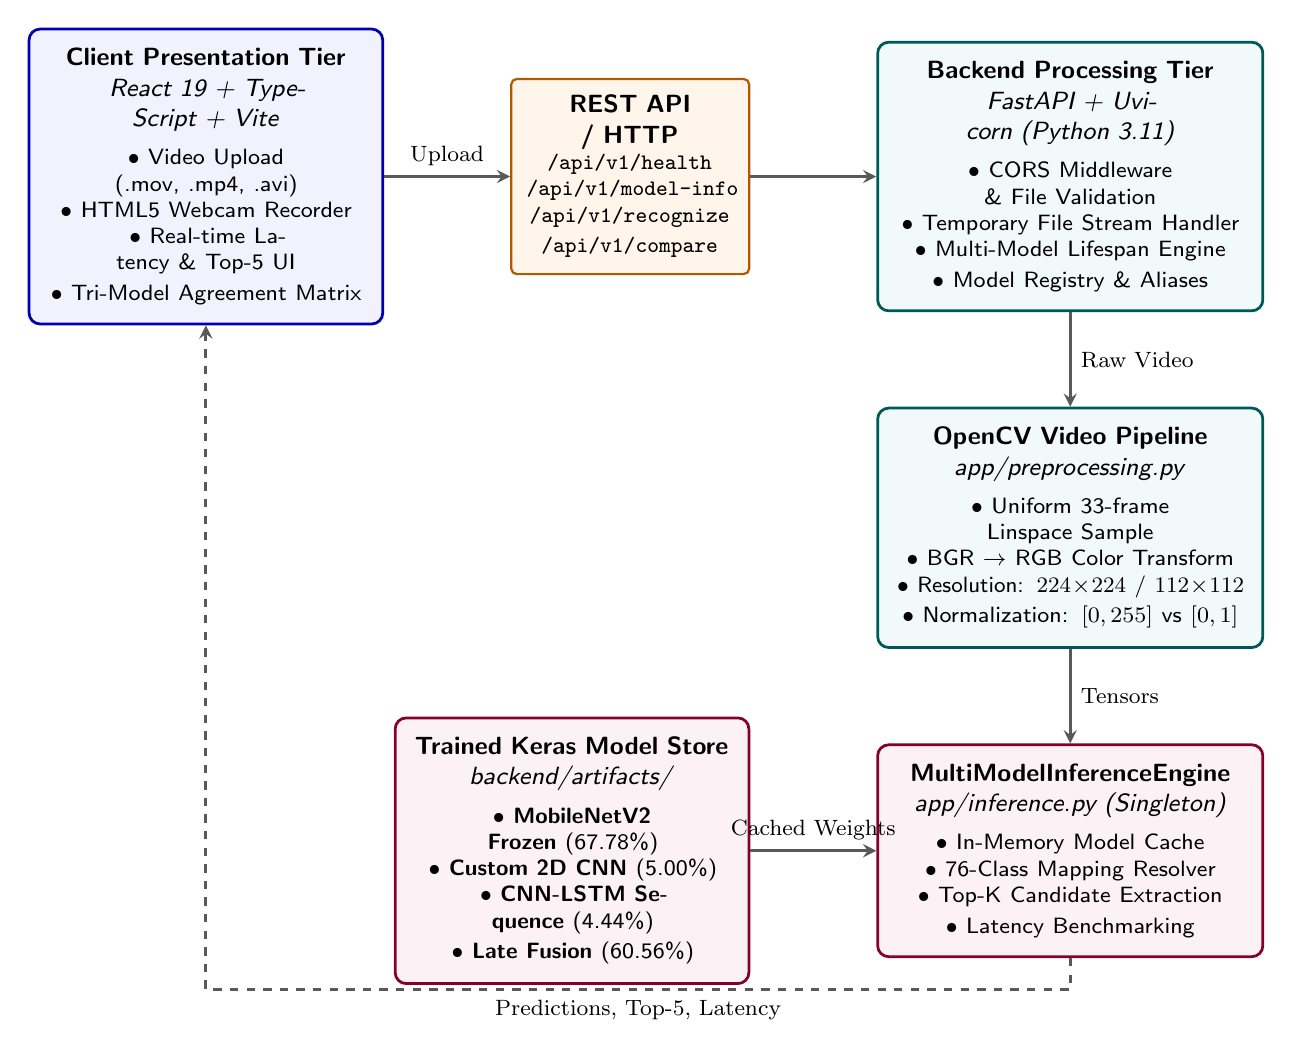
\begin{tikzpicture}[
    node distance=1.2cm and 1.5cm,
    font=\small\sffamily,
    box/.style={draw=blue!70!black, fill=blue!5, rounded corners=4pt, align=center, inner sep=7pt, line width=1pt},
    comp/.style={draw=teal!70!black, fill=teal!5, rounded corners=4pt, align=center, inner sep=7pt, line width=1pt},
    model/.style={draw=purple!70!black, fill=purple!5, rounded corners=4pt, align=center, inner sep=7pt, line width=1pt},
    data/.style={draw=orange!70!black, fill=orange!8, rounded corners=2pt, align=center, inner sep=6pt, line width=0.8pt},
    arrow/.style={->, >=stealth, line width=1.1pt, draw=gray!70!black}
]

% Client Tier
\node[box, text width=4.0cm] (client) {
    \textbf{Client Presentation Tier}\\
    \textit{React 19 + TypeScript + Vite}\\
    \vspace{0.15cm}
    \footnotesize
    $\bullet$ Video Upload (.mov, .mp4, .avi)\\
    $\bullet$ HTML5 Webcam Recorder\\
    $\bullet$ Real-time Latency \& Top-5 UI\\
    $\bullet$ Tri-Model Agreement Matrix
};

% REST Boundaries
\node[data, right=1.6cm of client, text width=2.6cm] (api) {
    \textbf{REST API / HTTP}\\
    \footnotesize
    \texttt{/api/v1/health}\\
    \texttt{/api/v1/model-info}\\
    \texttt{/api/v1/recognize}\\
    \texttt{/api/v1/compare}
};

% Backend Tier
\node[comp, right=1.6cm of api, text width=4.4cm] (backend) {
    \textbf{Backend Processing Tier}\\
    \textit{FastAPI + Uvicorn (Python 3.11)}\\
    \vspace{0.15cm}
    \footnotesize
    $\bullet$ CORS Middleware \& File Validation\\
    $\bullet$ Temporary File Stream Handler\\
    $\bullet$ Multi-Model Lifespan Engine\\
    $\bullet$ Model Registry \& Aliases
};

% Preprocessing Subsystem
\node[comp, below=1.2cm of backend, text width=4.4cm] (preproc) {
    \textbf{OpenCV Video Pipeline}\\
    \textit{app/preprocessing.py}\\
    \vspace{0.15cm}
    \footnotesize
    $\bullet$ Uniform 33-frame Linspace Sample\\
    $\bullet$ BGR $\to$ RGB Color Transform\\
    $\bullet$ Resolution: $224\times224$ / $112\times112$\\
    $\bullet$ Normalization: $[0, 255]$ vs $[0, 1]$
};

% Inference Engine Singleton
\node[model, below=1.2cm of preproc, text width=4.4cm] (engine) {
    \textbf{MultiModelInferenceEngine}\\
    \textit{app/inference.py (Singleton)}\\
    \vspace{0.15cm}
    \footnotesize
    $\bullet$ In-Memory Model Cache\\
    $\bullet$ 76-Class Mapping Resolver\\
    $\bullet$ Top-K Candidate Extraction\\
    $\bullet$ Latency Benchmarking
};

% Loaded Model Artifacts
\node[model, left=1.6cm of engine, text width=4.0cm] (models) {
    \textbf{Trained Keras Model Store}\\
    \textit{backend/artifacts/}\\
    \vspace{0.15cm}
    \footnotesize
    $\bullet$ \textbf{MobileNetV2 Frozen} (67.78\%)\\
    $\bullet$ \textbf{Custom 2D CNN} (5.00\%)\\
    $\bullet$ \textbf{CNN-LSTM Sequence} (4.44\%)\\
    $\bullet$ \textbf{Late Fusion} (60.56\%)
};

% Connectors
\draw[arrow] (client.east) -- node[above, font=\footnotesize] {Upload} (api.west);
\draw[arrow] (api.east) -- (backend.west);
\draw[arrow] (backend.south) -- node[right, font=\footnotesize] {Raw Video} (preproc.north);
\draw[arrow] (preproc.south) -- node[right, font=\footnotesize] {Tensors} (engine.north);
\draw[arrow] (models.east) -- node[above, font=\footnotesize] {Cached Weights} (engine.west);

% Response loop
\draw[arrow, dashed] (engine.south) -- ++(0,-0.4) -| node[near start, below, font=\footnotesize] {Predictions, Top-5, Latency} (client.south);

\end{tikzpicture}

\caption{SignBridge end-to-end system architecture, illustrating client presentation, FastAPI REST boundary, OpenCV preprocessing pipeline, and the cached multi-model inference engine.}
\label{fig:overall_arch}
\end{figure}

\section{Frontend Architecture}
\label{sec:frontend_architecture}
The frontend architecture is organized around modular React functional components, strictly typed TypeScript models, and centralized API communication services. The directory structure is organized as follows:
\begin{itemize}
    \item \texttt{src/components/layout/}: Contains foundational structural components, including the \texttt{Navbar} (which displays dynamic backend health badges and active model indicators) and the \texttt{Footer}.
    \item \texttt{src/components/dashboard/}: Implements the main informational hub, consisting of the \texttt{HeroSection}, the \texttt{ModelCards} component displaying evaluated architectures and benchmark accuracies, the \texttt{PipelineFlow} component, and the \texttt{VocabularyPreview} browser.
    \item \texttt{src/components/recognition/}: Houses the operational recognition workspace, including \texttt{VideoUploader} (drag-and-drop and file selection), \texttt{WebcamRecorder} (camera stream management, countdown timer, and blob generation), \texttt{VideoPreviewCard} (HTML5 video playback), and \texttt{RecognitionResultCard} (displaying predicted ISL words, confidence meters, latency badges, and top-5 probability rankings).
    \item \texttt{src/components/comparison/}: Contains the multi-model comparison suite, including \texttt{BenchmarkSummarySection}, \texttt{ModelComparisonCard}, and \texttt{AgreementAnalysisSection} for evaluating consensus and majority agreement across models.
    \item \texttt{src/services/recognitionApi.ts}: Provides strongly typed asynchronous HTTP client methods (\texttt{analyzeVideo}, \texttt{compareAllModels}, and \texttt{checkBackendHealth}) that communicate with the FastAPI backend.
    \item \texttt{src/types/index.ts}: Defines formal TypeScript interfaces for model metrics, prediction payloads, top-K candidates, and health responses, ensuring end-to-end type safety.
\end{itemize}

\section{Backend Architecture}
\label{sec:backend_architecture}
The backend architecture is structured around FastAPI's asynchronous application lifecycle, implemented across four core Python modules located in \texttt{backend/app/}:
\begin{enumerate}
    \item \texttt{config.py}: Defines global application constants, environment variable bindings, allowed video file extensions (\texttt{.mov}, \texttt{.mp4}, \texttt{.avi}, \texttt{.webm}), maximum upload size limits (100\,MB), frame sampling parameters ($N=33$), and the central \texttt{MODEL\_REGISTRY}. The registry defines metadata, target resolutions, normalizations, and filesystem paths for all registered models.
    \item \texttt{preprocessing.py}: Contains OpenCV video decoding and frame manipulation routines. The core functions \texttt{decode\_video\_frames} and \texttt{preprocess\_for\_model} enforce uniform temporal sampling via \texttt{np.linspace} and apply model-specific resizing and numerical scaling.
    \item \texttt{inference.py}: Implements the \texttt{MultiModelInferenceEngine} class as a global singleton. It manages the in-memory caching of loaded Keras models, loads the verified 76-class label mapping from JSON, computes normalized probability distributions, extracts top-$K$ candidate rankings, and performs equal-weight late fusion.
    \item \texttt{main.py}: Defines the FastAPI application instance, lifespan context manager for startup model pre-loading, CORS middleware configurations, and REST endpoint route handlers.
\end{enumerate}

\section{Model Inference Workflow}
\label{sec:inference_workflow}
The inference workflow translates an incoming raw video stream into a verified lexical sign prediction through five sequential stages, as illustrated in Figure \ref{fig:pipeline_flow}.

\begin{figure}[htbp]
\centering
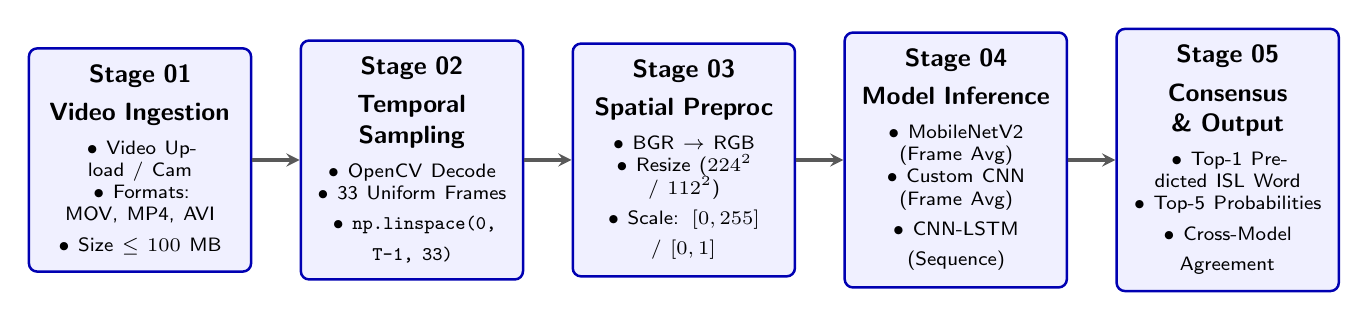
\begin{tikzpicture}[
    node distance=0.8cm and 0.5cm,
    font=\small\sffamily,
    stepbox/.style={draw=blue!70!black, fill=blue!6, rounded corners=3pt, align=center, inner sep=6pt, text width=2.4cm, line width=0.9pt},
    header/.style={font=\bfseries\footnotesize, text=blue!80!black},
    arrow/.style={->, >=stealth, line width=1.1pt, draw=gray!70!black}
]

\node[stepbox] (step1) {
    \textbf{Stage 01}\\[0.1cm]
    \textbf{Video Ingestion}\\[0.15cm]
    \scriptsize
    $\bullet$ Video Upload / Cam\\
    $\bullet$ Formats: MOV, MP4, AVI\\
    $\bullet$ Size $\le 100$ MB
};

\node[stepbox, right=0.6cm of step1] (step2) {
    \textbf{Stage 02}\\[0.1cm]
    \textbf{Temporal Sampling}\\[0.15cm]
    \scriptsize
    $\bullet$ OpenCV Decode\\
    $\bullet$ 33 Uniform Frames\\
    $\bullet$ \texttt{np.linspace(0, T-1, 33)}
};

\node[stepbox, right=0.6cm of step2] (step3) {
    \textbf{Stage 03}\\[0.1cm]
    \textbf{Spatial Preproc}\\[0.15cm]
    \scriptsize
    $\bullet$ BGR $\to$ RGB\\
    $\bullet$ Resize ($224^2$ / $112^2$)\\
    $\bullet$ Scale: $[0, 255]$ / $[0, 1]$
};

\node[stepbox, right=0.6cm of step3] (step4) {
    \textbf{Stage 04}\\[0.1cm]
    \textbf{Model Inference}\\[0.15cm]
    \scriptsize
    $\bullet$ MobileNetV2 (Frame Avg)\\
    $\bullet$ Custom CNN (Frame Avg)\\
    $\bullet$ CNN-LSTM (Sequence)
};

\node[stepbox, right=0.6cm of step4] (step5) {
    \textbf{Stage 05}\\[0.1cm]
    \textbf{Consensus \& Output}\\[0.15cm]
    \scriptsize
    $\bullet$ Top-1 Predicted ISL Word\\
    $\bullet$ Top-5 Probabilities\\
    $\bullet$ Cross-Model Agreement
};

\draw[arrow] (step1) -- (step2);
\draw[arrow] (step2) -- (step3);
\draw[arrow] (step3) -- (step4);
\draw[arrow] (step4) -- (step5);

\end{tikzpicture}

\caption{Five-stage inference pipeline flow in SignBridge, detailing ingestion, temporal linspace sampling, spatial standardization, model inference, and consensus output.}
\label{fig:pipeline_flow}
\end{figure}

The detailed operational mechanics of each stage are:
\begin{itemize}
    \item \textbf{Stage 1 (Video Ingestion)}: The user uploads an RGB video file or captures a clip via webcam. The backend validates the file extension and streams chunks into a named temporary file on disk while enforcing a 100\,MB ceiling.
    \item \textbf{Stage 2 (Uniform Frame Sampling)}: OpenCV opens the video container via \texttt{cv2.VideoCapture}. If the total frame count $T$ is readable, indices are generated via:
    \begin{equation}
        \mathcal{I} = \left\lfloor \text{linspace}(0, T - 1, 33) \right\rfloor \in \mathbb{Z}^{33}
        \label{eq:linspace}
    \end{equation}
    The capture pointer seeks directly to each index $\tau \in \mathcal{I}$, decoding the corresponding frame. If container metadata is missing, sequential decoding with linspace subsampling is executed as a fallback.
    \item \textbf{Stage 3 (Spatial Preprocessing)}: Each decoded frame is converted from BGR to RGB color-space and resized using \texttt{cv2.INTER\_AREA} interpolation to $224\times224$ (for MobileNetV2 and Custom CNN) or $112\times112$ (for CNN-LSTM). Numerical values are cast to float32 and scaled appropriately.
    \item \textbf{Stage 4 (Multi-Model Inference)}: The preprocessed tensor is routed to the selected model in the cached inference engine. Frame-level models compute forward passes across all 33 frames, while the recurrent CNN-LSTM evaluates the 5D sequence tensor directly.
    \item \textbf{Stage 5 (Consensus \& Aggregation)}: For frame-level architectures, the 33 frame probability vectors are averaged. The top predicted class index $\hat{k} = \arg\max_k \bar{p}_k$ is mapped to the corresponding ISL word label, top-5 candidates are extracted, and cross-model agreement metrics are computed.
\end{itemize}

\section{API Communication and Protocols}
\label{sec:api_communication}
Communication between the React client and FastAPI backend occurs over standard HTTP/1.1 protocols using JSON and Multipart Form-Data encodings. Table \ref{tab:api_endpoints_summary} outlines the primary API endpoints exposed by the SignBridge backend.

\begin{table}[htbp]
\centering
\caption{SignBridge REST API endpoint specifications.}
\label{tab:api_endpoints_summary}
\small
\begin{tabularx}{\textwidth}{l l p{4.2cm} X}
\toprule
\textbf{HTTP Method} & \textbf{Endpoint Path} & \textbf{Request Payload} & \textbf{Response Description} \\
\midrule
\texttt{GET} & \texttt{/api/v1/health} & None & Returns service health status, class count (76), default model ID, and load status per registered model. \\
\addlinespace
\texttt{GET} & \texttt{/api/v1/model-info} & Optional query: \texttt{?model=<id>} & Returns architecture specifications, input/output tensor shapes, and preprocessing parameters. \\
\addlinespace
\texttt{POST} & \texttt{/api/v1/recognize} & \texttt{multipart/form-data}: \texttt{video} (File), \texttt{model} (Form/Query string) & Decodes video, runs inference on specified model, and returns top-1 word, confidence, top-5 candidates, and latency. \\
\addlinespace
\texttt{POST} & \texttt{/api/v1/compare} & \texttt{multipart/form-data}: \texttt{video} (File) & Evaluates all three models in parallel on the same clip; returns individual predictions, latencies, and consensus metrics. \\
\bottomrule
\end{tabularx}
\end{table}

\section{Data Flow}
\label{sec:data_flow}
Data traverses the SignBridge pipeline through tightly defined representations:
\begin{enumerate}
    \item \textbf{Binary Video Bitstream}: Raw compressed video packets (\texttt{.MOV}, \texttt{.mp4}, \texttt{.webm}) arrive from the browser and are written to a temporary storage path on the backend host.
    \item \textbf{Decoded Raw Frame List}: A Python list of 33 NumPy arrays of shape $(H, W, 3)$ with \texttt{uint8} values in $[0, 255]$ in RGB color order.
    \item \textbf{Preprocessed Model Tensor}:
    \begin{itemize}
        \item For MobileNetV2: 4D array of shape $(33, 224, 224, 3)$ of type \texttt{float32} in range $[0, 255]$.
        \item For Custom CNN: 4D array of shape $(33, 224, 224, 3)$ of type \texttt{float32} in range $[0, 1]$.
        \item For CNN-LSTM: 5D array of shape $(1, 33, 112, 112, 3)$ of type \texttt{float32} in range $[0, 1]$.
    \end{itemize}
    \item \textbf{Logit and Softmax Distributions}: Raw neural output tensors transformed by the terminal Softmax activation into a discrete probability distribution over 76 classes, satisfying $\sum_{k=1}^{76} p_k = 1.0$.
    \item \textbf{Structured JSON Payload}: Serialized JSON response containing predicted lexical words, floating-point confidence values, top-$K$ candidate arrays, and execution timing metrics.
\end{enumerate}

\section{System Workflow}
\label{sec:system_workflow}
Figure \ref{fig:workflow_frontend} illustrates the complete user interaction workflow implemented in the frontend application, showing validation checkpoints, mode selection, and error-handling pathways.

\begin{figure}[htbp]
\centering
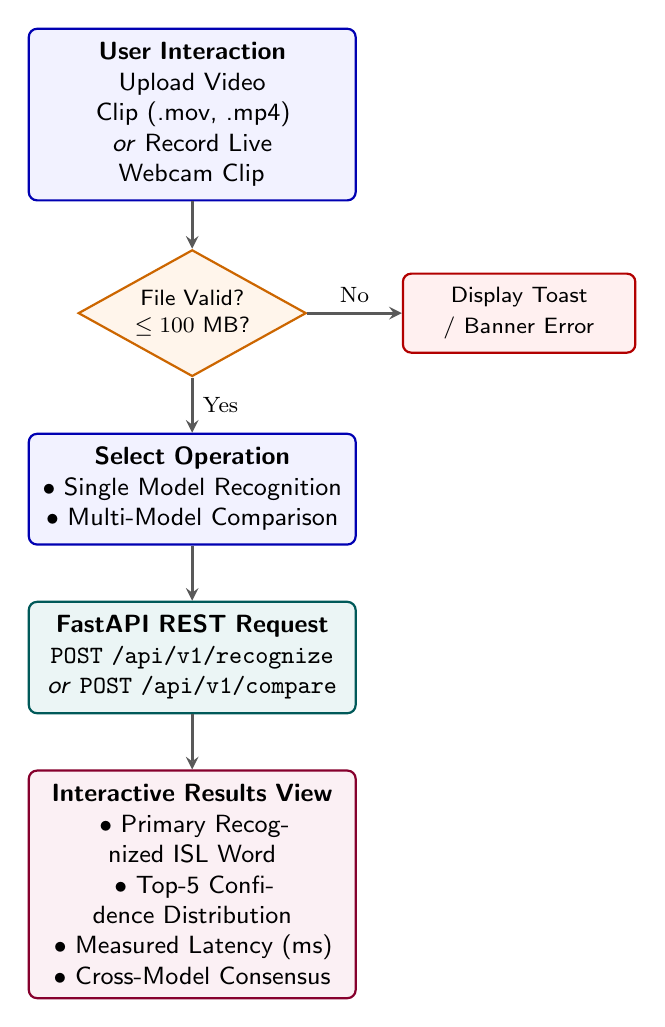
\begin{tikzpicture}[
    node distance=0.8cm and 1.2cm,
    font=\small\sffamily,
    action/.style={draw=blue!70!black, fill=blue!5, rounded corners=3pt, align=center, inner sep=5pt, text width=3.8cm, line width=0.8pt},
    decision/.style={draw=orange!80!black, fill=orange!8, diamond, aspect=1.8, align=center, inner sep=2pt, font=\footnotesize\sffamily, line width=0.8pt},
    service/.style={draw=teal!70!black, fill=teal!8, rounded corners=3pt, align=center, inner sep=5pt, text width=3.8cm, line width=0.8pt},
    ui/.style={draw=purple!70!black, fill=purple!6, rounded corners=3pt, align=center, inner sep=5pt, text width=3.8cm, line width=0.8pt},
    arrow/.style={->, >=stealth, line width=1pt, draw=gray!70!black}
]

\node[action] (input) {
    \textbf{User Interaction}\\
    Upload Video Clip (.mov, .mp4)\\
    \textit{or} Record Live Webcam Clip
};

\node[decision, below=0.6cm of input] (val) {
    File Valid?\\
    $\le 100$ MB?
};

\node[action, right=1.2cm of val, text width=2.6cm, draw=red!70!black, fill=red!6] (err) {
    \footnotesize Display Toast / Banner Error
};

\node[action, below=0.7cm of val] (mode) {
    \textbf{Select Operation}\\
    $\bullet$ Single Model Recognition\\
    $\bullet$ Multi-Model Comparison
};

\node[service, below=0.7cm of mode] (api) {
    \textbf{FastAPI REST Request}\\
    \texttt{POST /api/v1/recognize}\\
    \textit{or} \texttt{POST /api/v1/compare}
};

\node[ui, below=0.7cm of api] (result) {
    \textbf{Interactive Results View}\\
    $\bullet$ Primary Recognized ISL Word\\
    $\bullet$ Top-5 Confidence Distribution\\
    $\bullet$ Measured Latency (ms)\\
    $\bullet$ Cross-Model Consensus
};

\draw[arrow] (input) -- (val);
\draw[arrow] (val) -- node[above, font=\footnotesize] {No} (err);
\draw[arrow] (val) -- node[right, font=\footnotesize] {Yes} (mode);
\draw[arrow] (mode) -- (api);
\draw[arrow] (api) -- (result);

\end{tikzpicture}

\caption{SignBridge frontend user interaction and execution workflow, from file selection or webcam capture through client validation, REST dispatch, and results visualization.}
\label{fig:workflow_frontend}
\end{figure}

The user may either drag-and-drop an existing sign video clip or record a live clip using their webcam. The client performs instant format and size verification; if valid, the user chooses between single-model recognition or the tri-model comparison suite. Upon receiving the JSON response, the frontend renders interactive confidence meters, candidate lists, and agreement banners.

\chapter{Dataset and Preprocessing}
\label{ch:dataset}

\section{Dataset Description and Vocabulary}
\label{sec:dataset_desc}
SignBridge is trained and evaluated on an isolated dynamic Indian Sign Language (ISL) video corpus. Each recording captures an individual signer executing a single sign gesture in QuickTime (\texttt{.MOV}) or MPEG-4 (\texttt{.mp4}) format. The dataset encompasses \textbf{76 discrete lexical sign classes} across 1,166 video recordings ($\approx 15.3$ samples per class). Table \ref{tab:verified_classes} lists the complete 76-class vocabulary from the ground-truth mapping artifact (\texttt{class\_mapping.json}).

\begin{table}[htbp]
\centering
\caption{Complete 76-class Indian Sign Language vocabulary mapping.}
\label{tab:verified_classes}
\tiny
\setlength{\tabcolsep}{3pt}
\renewcommand{\arraystretch}{0.92}
\begin{tabularx}{\textwidth}{c l c l c l c l}
\toprule
\textbf{Idx} & \textbf{Word} & \textbf{Idx} & \textbf{Word} & \textbf{Idx} & \textbf{Word} & \textbf{Idx} & \textbf{Word} \\
\midrule
0 & \texttt{afternoon} & 19 & \texttt{famous} & 38 & \texttt{month} & 57 & \texttt{small} \\
1 & \texttt{animal} & 20 & \texttt{fast} & 39 & \texttt{morning} & 58 & \texttt{suit} \\
2 & \texttt{bad} & 21 & \texttt{female} & 40 & \texttt{mouse} & 59 & \texttt{sunday} \\
3 & \texttt{beautiful} & 22 & \texttt{fish} & 41 & \texttt{narrow} & 60 & \texttt{t\_shirt} \\
4 & \texttt{big} & 23 & \texttt{flat} & 42 & \texttt{new} & 61 & \texttt{tall} \\
5 & \texttt{bird} & 24 & \texttt{friday} & 43 & \texttt{night} & 62 & \texttt{thursday} \\
6 & \texttt{blind} & 25 & \texttt{good} & 44 & \texttt{old} & 63 & \texttt{time} \\
7 & \texttt{cat} & 26 & \texttt{happy} & 45 & \texttt{pant} & 64 & \texttt{today} \\
8 & \texttt{cheap} & 27 & \texttt{hat} & 46 & \texttt{pocket} & 65 & \texttt{tomorrow} \\
9 & \texttt{clothing} & 28 & \texttt{healthy} & 47 & \texttt{quiet} & 66 & \texttt{tuesday} \\
10 & \texttt{cold} & 29 & \texttt{horse} & 48 & \texttt{sad} & 67 & \texttt{ugly} \\
11 & \texttt{cow} & 30 & \texttt{hot} & 49 & \texttt{saturday} & 68 & \texttt{warm} \\
12 & \texttt{curved} & 31 & \texttt{hour} & 50 & \texttt{second} & 69 & \texttt{wednesday} \\
13 & \texttt{deaf} & 32 & \texttt{light} & 51 & \texttt{shirt} & 70 & \texttt{week} \\
14 & \texttt{dog} & 33 & \texttt{long} & 52 & \texttt{shoes} & 71 & \texttt{wet} \\
15 & \texttt{dress} & 34 & \texttt{loose} & 53 & \texttt{short} & 72 & \texttt{wide} \\
16 & \texttt{dry} & 35 & \texttt{loud} & 54 & \texttt{sick} & 73 & \texttt{year} \\
17 & \texttt{evening} & 36 & \texttt{minute} & 55 & \texttt{skirt} & 74 & \texttt{yesterday} \\
18 & \texttt{expensive} & 37 & \texttt{monday} & 56 & \texttt{slow} & 75 & \texttt{young} \\
\bottomrule
\end{tabularx}
\end{table}

\section{Dataset Organization and Splits}
\label{sec:dataset_splits}
The 1,166 video samples are organized by class directory and partitioned into strictly disjoint training, validation, and held-out test splits, detailed in Table \ref{tab:dataset_splits}. The 180-video held-out test set is strictly sequestered during training.

\begin{table}[htbp]
\centering
\caption{Dataset partitioning across training, validation, and test splits.}
\label{tab:dataset_splits}
\scriptsize
\begin{tabularx}{\textwidth}{l r r X}
\toprule
\textbf{Split Partition} & \textbf{Video Count} & \textbf{Percentage} & \textbf{Operational Role} \\
\midrule
\textbf{Training Split} & 806 & 69.12\% & Model weight optimization via mini-batch gradient descent. \\
\textbf{Validation Split} & 180 & 15.44\% & Hyperparameter tuning, learning rate scheduling, and early stopping. \\
\textbf{Held-Out Test Split} & 180 & 15.44\% & Final unbiased evaluation of test accuracy and Macro $F_1$. \\
\midrule
\textbf{Total Corpus} & \textbf{1,166} & \textbf{100.00\%} & Complete multi-class ISL video corpus across 76 classes. \\
\bottomrule
\end{tabularx}
\end{table}

\section{Uniform Frame Sampling and Spatial Preprocessing}
\label{sec:frame_sampling}
Because raw videos have varying frame rates and durations (1.5 to 4.0\,s), fixed-rate sampling induces variable sequence lengths. SignBridge enforces \textbf{Uniform Temporal Linspace Sampling}, extracting exactly $N = 33$ frames per clip:
\begin{equation}
    \mathcal{I} = \left\{ \left\lfloor \frac{i \cdot (T - 1)}{N - 1} \right\rfloor \;\middle|\; i = 0, 1, \dots, N - 1 \right\} \subset \{0, 1, \dots, T - 1\}
    \label{eq:linspace_sampling}
\end{equation}
Extracted frames are converted from BGR to RGB and resized using OpenCV's area-based interpolation (\texttt{cv2.INTER\_AREA}) to avoid downsampling aliasing \cite{bradski2000opencv}.

\section{Normalization and Model Tensor Representation}
\label{sec:normalization}
Table \ref{tab:preproc_specs} summarizes the model-specific input tensors. MobileNetV2 retains raw $[0, 255]$ values as it embeds an internal Keras \texttt{Rescaling} layer ($x/127.5 - 1 \in [-1, 1]$), while Custom CNN and CNN-LSTM inputs are scaled to $[0, 1]$ via division by 255.0.

\begin{table}[htbp]
\centering
\caption{Model-specific input tensor specifications and normalization.}
\label{tab:preproc_specs}
\scriptsize
\begin{tabularx}{\textwidth}{l c c c X}
\toprule
\textbf{Model Target} & \textbf{Tensor Shape} & \textbf{Resolution} & \textbf{Input Domain} & \textbf{Normalization Scheme} \\
\midrule
\textbf{MobileNetV2} & $(33, 224, 224, 3)$ & $224\times224$ & $[0, 255]$ float32 & Internal \texttt{Rescaling} layer: $x \mapsto \frac{x}{127.5}-1 \in [-1, 1]$. \\
\textbf{Custom 2D CNN} & $(33, 224, 224, 3)$ & $224\times224$ & $[0, 1]$ float32 & Direct division by 255.0 prior to model entry. \\
\textbf{CNN-LSTM} & $(1, 33, 112, 112, 3)$ & $112\times112$ & $[0, 1]$ float32 & Direct division by 255.0; 5D tensor with batch dimension. \\
\bottomrule
\end{tabularx}
\end{table}

\chapter{Methodology and Model Implementation}
\label{ch:methodology}

\section{Overall Recognition Pipeline}
\label{sec:overall_pipeline}
The core methodology of SignBridge addresses dynamic Indian Sign Language recognition through a comparative machine learning framework. Recognizing that dynamic sign language conveys meaning through both static hand configurations (spatial features) and gesture trajectories (temporal sequences), three distinct deep learning architectures were designed, trained, and benchmarked on identical 76-class dataset splits:
\begin{enumerate}
    \item \textbf{Transfer Learning with Frozen Spatial Backbone}: MobileNetV2 with ImageNet weights, evaluated via multi-frame temporal probability averaging.
    \item \textbf{Scratch 2D Convolutional Baseline}: A custom 3-block 2D CNN trained from scratch with spatial data augmentation and multi-frame averaging.
    \item \textbf{Joint Spatio-Temporal Sequential Model}: A CNN-LSTM pairing TimeDistributed convolutional feature extractors with a recurrent Long Short-Term Memory network.
\end{enumerate}

\section{MobileNetV2 and Transfer Learning}
\label{sec:mobilenetv2_arch}
MobileNetV2 \cite{sandler2018mobilenetv2} serves as the primary recognition engine in SignBridge. Rather than training visual feature extractors from scratch on limited sign video data, transfer learning leverages rich generic visual representations acquired by training on the massive ImageNet database \cite{deng2009imagenet}.

\subsection{Architectural Details and Layer Configuration}
The complete architecture of the implemented MobileNetV2 model (\texttt{SignBridge\_MobileNetV2\_Frozen}) is depicted in Figure \ref{fig:mobilenetv2_arch}.

\begin{figure}[htbp]
\centering
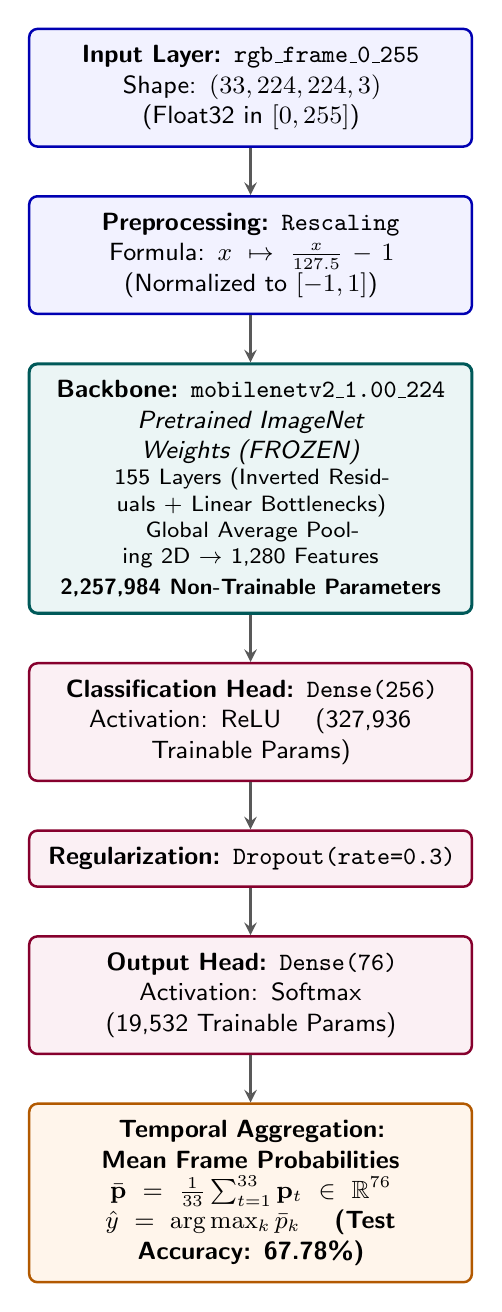
\begin{tikzpicture}[
    node distance=0.9cm and 1.2cm,
    font=\small\sffamily,
    layer/.style={draw=blue!70!black, fill=blue!5, rounded corners=3pt, align=center, inner sep=6pt, text width=5.2cm, line width=0.9pt},
    frozen/.style={draw=teal!70!black, fill=teal!8, rounded corners=3pt, align=center, inner sep=6pt, text width=5.2cm, line width=1.1pt},
    head/.style={draw=purple!70!black, fill=purple!6, rounded corners=3pt, align=center, inner sep=6pt, text width=5.2cm, line width=0.9pt},
    agg/.style={draw=orange!70!black, fill=orange!8, rounded corners=3pt, align=center, inner sep=6pt, text width=5.2cm, line width=0.9pt},
    arrow/.style={->, >=stealth, line width=1pt, draw=gray!70!black}
]

\node[layer] (in) {
    \textbf{Input Layer: \texttt{rgb\_frame\_0\_255}}\\
    Shape: $(33, 224, 224, 3)$ \quad (Float32 in $[0, 255]$)
};

\node[layer, below=0.6cm of in] (rescale) {
    \textbf{Preprocessing: \texttt{Rescaling}}\\
    Formula: $x \mapsto \frac{x}{127.5} - 1$ \quad (Normalized to $[-1, 1]$)
};

\node[frozen, below=0.6cm of rescale] (backbone) {
    \textbf{Backbone: \texttt{mobilenetv2\_1.00\_224}}\\
    \textit{Pretrained ImageNet Weights (FROZEN)}\\
    \footnotesize
    155 Layers (Inverted Residuals + Linear Bottlenecks)\\
    Global Average Pooling 2D $\to$ 1,280 Features\\
    \textbf{2,257,984 Non-Trainable Parameters}
};

\node[head, below=0.6cm of backbone] (dense1) {
    \textbf{Classification Head: \texttt{Dense(256)}}\\
    Activation: ReLU \quad (327,936 Trainable Params)
};

\node[head, below=0.6cm of dense1] (drop) {
    \textbf{Regularization: \texttt{Dropout(rate=0.3)}}
};

\node[head, below=0.6cm of drop] (dense2) {
    \textbf{Output Head: \texttt{Dense(76)}}\\
    Activation: Softmax \quad (19,532 Trainable Params)
};

\node[agg, below=0.6cm of dense2] (agg) {
    \textbf{Temporal Aggregation: Mean Frame Probabilities}\\
    $\bar{\mathbf{p}} = \frac{1}{33} \sum_{t=1}^{33} \mathbf{p}_t \in \mathbb{R}^{76}$\\
    $\hat{y} = \arg\max_k \bar{p}_k$ \quad \textbf{(Test Accuracy: 67.78\%)}
};

\draw[arrow] (in) -- (rescale);
\draw[arrow] (rescale) -- (backbone);
\draw[arrow] (backbone) -- (dense1);
\draw[arrow] (dense1) -- (drop);
\draw[arrow] (drop) -- (dense2);
\draw[arrow] (dense2) -- (agg);

\end{tikzpicture}

\caption{Architectural layout of the MobileNetV2 transfer learning model in SignBridge, showing the frozen ImageNet backbone, custom dense classification head, and multi-frame probability averaging.}
\label{fig:mobilenetv2_arch}
\end{figure}

The model comprises four principal functional stages:
\begin{enumerate}
    \item \textbf{Input Layer (\texttt{rgb\_frame\_0\_255})}: Accepts 4D RGB frame tensors of shape $(\text{None}, 224, 224, 3)$ with \texttt{float32} values in the raw pixel range $[0, 255]$.
    \item \textbf{Preprocessing Layer (\texttt{mobilenetv2\_preprocessing})}: An internal Keras \texttt{Rescaling} layer that normalizes input pixel values into the range $[-1.0, 1.0]$ via the linear transformation:
    \begin{equation}
        x_{\text{norm}} = \frac{x}{127.5} - 1.0
        \label{eq:mobilenet_rescale}
    \end{equation}
    Embedding this layer directly inside the model graph ensures that inference clients can feed raw $[0, 255]$ frames without external numerical drift.
    \item \textbf{Frozen Feature Backbone (\texttt{mobilenetv2\_1.00\_224})}: The standard MobileNetV2 architecture with width multiplier $\alpha = 1.0$, initialized with pre-trained ImageNet weights. The backbone contains 155 structural layers consisting of inverted residual blocks with depthwise separable convolutions and linear bottlenecks. All backbone weights are strictly frozen (\texttt{trainable=False}), holding \textbf{2,257,984 parameters} non-trainable. The backbone terminates in a Global Average Pooling 2D operation, producing a compact 1,280-dimensional visual feature embedding.
    \item \textbf{Custom Trainable Classification Head (\texttt{frozen\_mobilenetv2\_head})}: A sequential classification sub-network attached to the 1,280-dimensional feature output:
    \begin{itemize}
        \item \texttt{Dense(256, activation='relu')}: Fully connected layer projecting 1,280 features into 256 dimensions, introducing non-linear feature combination ($1280 \times 256 + 256 = 327,936$ trainable parameters).
        \item \texttt{Dropout(rate=0.3)}: Regularization layer that randomly zeroes 30\% of hidden units during training to prevent co-adaptation \cite{srivastava2014dropout}.
        \item \texttt{Dense(76, activation='softmax')}: Terminal classification layer projecting 256 units to 76 class logits transformed into a probability distribution via Softmax ($256 \times 76 + 76 = 19,532$ trainable parameters).
    \end{itemize}
\end{enumerate}

Table \ref{tab:mobilenetv2_params} summarizes the verified parameter counts of the MobileNetV2 model artifact (\texttt{mobilenetv2\_frozen\_best.keras}, file size 13.8\,MB).

\begin{table}[htbp]
\centering
\caption{Verified layer and parameter summary for MobileNetV2 (Frozen Backbone).}
\label{tab:mobilenetv2_params}
\small
\begin{tabularx}{\textwidth}{l l c r X}
\toprule
\textbf{Layer Name} & \textbf{Layer Type} & \textbf{Output Shape} & \textbf{Param \#} & \textbf{Trainable Status} \\
\midrule
\texttt{rgb\_frame\_0\_255} & InputLayer & $(\text{None}, 224, 224, 3)$ & 0 & Non-trainable \\
\texttt{mobilenetv2\_preprocessing} & Rescaling & $(\text{None}, 224, 224, 3)$ & 0 & Non-trainable \\
\texttt{mobilenetv2\_1.00\_224} & Functional Backbone & $(\text{None}, 1280)$ & 2,257,984 & Frozen (ImageNet) \\
\texttt{dense} & Dense (ReLU) & $(\text{None}, 256)$ & 327,936 & Trainable \\
\texttt{dropout} & Dropout ($p=0.3$) & $(\text{None}, 256)$ & 0 & Active in training \\
\texttt{dense\_1} & Dense (Softmax) & $(\text{None}, 76)$ & 19,532 & Trainable \\
\midrule
\textbf{Total Parameters} & \multicolumn{2}{l}{\textbf{2,605,452} (9.94\,MB)} & \multicolumn{2}{l}{\textbf{Trainable: 347,468} (1.33\,MB)} \\
\textbf{Non-Trainable} & \multicolumn{4}{l}{\textbf{2,257,984} (8.61\,MB, 86.66\% of network)} \\
\bottomrule
\end{tabularx}
\end{table}

\subsection{Temporal Aggregation Mechanism}
During inference, a video clip is represented by its 33 uniformly sampled frames $\mathbf{X} = \{I_1, I_2, \dots, I_{33}\} \subset \mathbb{R}^{33 \times 224 \times 224 \times 3}$. The model executes a batched forward pass over all 33 frames simultaneously, producing a sequence of frame-level probability vectors:
\begin{equation}
    \mathbf{p}_t = \text{Softmax}(\text{Model}(I_t)) \in \mathbb{R}^{76}, \quad t = 1, 2, \dots, 33
    \label{eq:frame_prob}
\end{equation}
The aggregated video-level probability vector $\bar{\mathbf{p}}$ is computed by averaging the frame-level distributions across the entire temporal sequence:
\begin{equation}
    \bar{\mathbf{p}} = \frac{1}{33} \sum_{t=1}^{33} \mathbf{p}_t \in \mathbb{R}^{76}
    \label{eq:mean_prob}
\end{equation}
The predicted lexical sign class $\hat{y}$ is selected via the argmax operator:
\begin{equation}
    \hat{y} = \arg\max_{k \in \{0, \dots, 75\}} \bar{p}_k
    \label{eq:predicted_class}
\end{equation}
This multi-frame probability averaging strategy provides strong spatial robustness: noise, motion blur, or partial hand occlusions in isolated frames are smoothly mitigated by confident predictions across the remainder of the clip.

\subsection{Strengths and Limitations}
\begin{itemize}
    \item \textbf{Strengths}: Superior sample efficiency on small datasets; frozen pre-trained weights eliminate overfitting; compact model size (13.8\,MB); fast CPU forward pass ($\approx 140$\,ms per 33-frame batch).
    \item \textbf{Limitations}: Does not model strict temporal ordering or frame velocity transitions; treats the 33 frames as an unordered set during probability averaging.
\end{itemize}

\section{Custom 2D CNN Architecture (Baseline)}
\label{sec:custom_cnn_arch}
To evaluate how effectively a convolutional network can learn sign language features entirely from scratch without external pre-training, a baseline 3-block 2D CNN (\texttt{SignBridge\_CNN}) was implemented.

\subsection{Architectural Details and Layer Configuration}
The architectural topology of the Custom 2D CNN is illustrated in Figure \ref{fig:custom_cnn_arch}.

\begin{figure}[htbp]
\centering
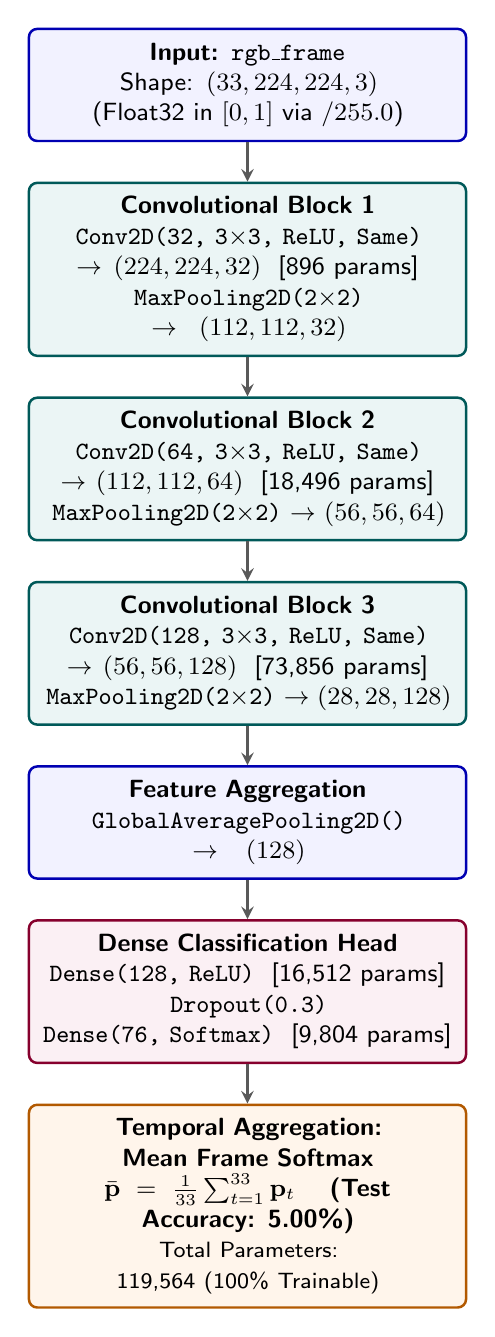
\begin{tikzpicture}[
    node distance=0.7cm and 1.2cm,
    font=\small\sffamily,
    layer/.style={draw=blue!70!black, fill=blue!5, rounded corners=3pt, align=center, inner sep=5pt, text width=5.2cm, line width=0.9pt},
    conv/.style={draw=teal!70!black, fill=teal!8, rounded corners=3pt, align=center, inner sep=5pt, text width=5.2cm, line width=0.9pt},
    dense/.style={draw=purple!70!black, fill=purple!6, rounded corners=3pt, align=center, inner sep=5pt, text width=5.2cm, line width=0.9pt},
    agg/.style={draw=orange!70!black, fill=orange!8, rounded corners=3pt, align=center, inner sep=5pt, text width=5.2cm, line width=0.9pt},
    arrow/.style={->, >=stealth, line width=1pt, draw=gray!70!black}
]

\node[layer] (in) {
    \textbf{Input: \texttt{rgb\_frame}}\\
    Shape: $(33, 224, 224, 3)$ \quad (Float32 in $[0, 1]$ via $/ 255.0$)
};

\node[conv, below=0.5cm of in] (block1) {
    \textbf{Convolutional Block 1}\\
    \texttt{Conv2D(32, 3$\times$3, ReLU, Same)} $\to (224, 224, 32)$ \ [896 params]\\
    \texttt{MaxPooling2D(2$\times$2)} $\to (112, 112, 32)$
};

\node[conv, below=0.5cm of block1] (block2) {
    \textbf{Convolutional Block 2}\\
    \texttt{Conv2D(64, 3$\times$3, ReLU, Same)} $\to (112, 112, 64)$ \ [18,496 params]\\
    \texttt{MaxPooling2D(2$\times$2)} $\to (56, 56, 64)$
};

\node[conv, below=0.5cm of block2] (block3) {
    \textbf{Convolutional Block 3}\\
    \texttt{Conv2D(128, 3$\times$3, ReLU, Same)} $\to (56, 56, 128)$ \ [73,856 params]\\
    \texttt{MaxPooling2D(2$\times$2)} $\to (28, 28, 128)$
};

\node[layer, below=0.5cm of block3] (gap) {
    \textbf{Feature Aggregation}\\
    \texttt{GlobalAveragePooling2D()} $\to (128)$
};

\node[dense, below=0.5cm of gap] (dense1) {
    \textbf{Dense Classification Head}\\
    \texttt{Dense(128, ReLU)} \ [16,512 params]\\
    \texttt{Dropout(0.3)}\\
    \texttt{Dense(76, Softmax)} \ [9,804 params]
};

\node[agg, below=0.5cm of dense1] (agg) {
    \textbf{Temporal Aggregation: Mean Frame Softmax}\\
    $\bar{\mathbf{p}} = \frac{1}{33} \sum_{t=1}^{33} \mathbf{p}_t$ \quad \textbf{(Test Accuracy: 5.00\%)}\\
    \footnotesize Total Parameters: 119,564 (100\% Trainable)
};

\draw[arrow] (in) -- (block1);
\draw[arrow] (block1) -- (block2);
\draw[arrow] (block2) -- (block3);
\draw[arrow] (block3) -- (gap);
\draw[arrow] (gap) -- (dense1);
\draw[arrow] (dense1) -- (agg);

\end{tikzpicture}

\caption{Architectural layout of the Custom 2D CNN baseline in SignBridge, detailing convolutional filter blocks, spatial max-pooling, global average pooling, and classification head.}
\label{fig:custom_cnn_arch}
\end{figure}

The network processes 4D tensors of shape $(\text{None}, 224, 224, 3)$ with values normalized into $[0, 1]$ float32:
\begin{enumerate}
    \item \textbf{Training Augmentation Sub-network (\texttt{training\_augmentation})}: A sequential data augmentation container active only during training, incorporating:
    \begin{itemize}
        \item \texttt{RandomRotation(factor=0.04)}: Slight rotation simulating camera or signer tilt.
        \item \texttt{RandomZoom(height\_factor=0.08, width\_factor=0.08)}: Simulating minor scale variation.
        \item \texttt{RandomTranslation(height\_factor=0.06, width\_factor=0.06)}: Spatial jitter.
    \end{itemize}
    At inference time, this layer acts as an identity pass-through.
    \item \textbf{Convolutional Block 1}:
    \begin{itemize}
        \item \texttt{conv\_1}: \texttt{Conv2D(32, (3, 3), padding='same', activation='relu')}. Produces $(\text{None}, 224, 224, 32)$ with $(3 \times 3 \times 3 + 1) \times 32 = 896$ parameters.
        \item \texttt{pool\_1}: \texttt{MaxPooling2D(pool\_size=(2, 2))}. Downsamples spatial resolution to $(\text{None}, 112, 112, 32)$.
    \end{itemize}
    \item \textbf{Convolutional Block 2}:
    \begin{itemize}
        \item \texttt{conv\_2}: \texttt{Conv2D(64, (3, 3), padding='same', activation='relu')}. Produces $(\text{None}, 112, 112, 64)$ with $(3 \times 3 \times 32 + 1) \times 64 = 18,496$ parameters.
        \item \texttt{pool\_2}: \texttt{MaxPooling2D(pool\_size=(2, 2))}. Downsamples to $(\text{None}, 56, 56, 64)$.
    \end{itemize}
    \item \textbf{Convolutional Block 3}:
    \begin{itemize}
        \item \texttt{conv\_3}: \texttt{Conv2D(128, (3, 3), padding='same', activation='relu')}. Produces $(\text{None}, 56, 56, 128)$ with $(3 \times 3 \times 64 + 1) \times 128 = 73,856$ parameters.
        \item \texttt{pool\_3}: \texttt{MaxPooling2D(pool\_size=(2, 2))}. Downsamples to $(\text{None}, 28, 28, 128)$.
    \end{itemize}
    \item \textbf{Global Feature Aggregation}:
    \begin{itemize}
        \item \texttt{global\_average\_pooling2d}: Collapses spatial dimensions $(28 \times 28)$ into a single 128-dimensional vector by computing the spatial mean for each channel, avoiding the parameter explosion associated with flattening.
    \end{itemize}
    \item \textbf{Dense Classification Head}:
    \begin{itemize}
        \item \texttt{dense}: \texttt{Dense(128, activation='relu')}. $128 \times 128 + 128 = 16,512$ parameters.
        \item \texttt{dropout}: \texttt{Dropout(rate=0.3)}.
        \item \texttt{word\_classification}: \texttt{Dense(76, activation='softmax')}. $128 \times 76 + 76 = 9,804$ parameters.
    \end{itemize}
\end{enumerate}

Table \ref{tab:custom_cnn_params} details the complete layer parameters for the Custom 2D CNN (\texttt{cnn\_baseline\_best.keras}, file size 1.50\,MB).

\begin{table}[htbp]
\centering
\caption{Verified layer and parameter summary for Custom 2D CNN (Baseline).}
\label{tab:custom_cnn_params}
\small
\begin{tabularx}{\textwidth}{l l c r X}
\toprule
\textbf{Layer Name} & \textbf{Layer Type} & \textbf{Output Shape} & \textbf{Param \#} & \textbf{Description} \\
\midrule
\texttt{rgb\_frame} & InputLayer & $(\text{None}, 224, 224, 3)$ & 0 & Normalized $[0, 1]$ RGB frames \\
\texttt{training\_augmentation} & Sequential & $(\text{None}, 224, 224, 3)$ & 0 & Rotation, zoom, translation (training only) \\
\texttt{conv\_1} & Conv2D & $(\text{None}, 224, 224, 32)$ & 896 & 32 filters, $3\times3$, ReLU \\
\texttt{pool\_1} & MaxPooling2D & $(\text{None}, 112, 112, 32)$ & 0 & $2\times2$ spatial max pooling \\
\texttt{conv\_2} & Conv2D & $(\text{None}, 112, 112, 64)$ & 18,496 & 64 filters, $3\times3$, ReLU \\
\texttt{pool\_2} & MaxPooling2D & $(\text{None}, 56, 56, 64)$ & 0 & $2\times2$ spatial max pooling \\
\texttt{conv\_3} & Conv2D & $(\text{None}, 56, 56, 128)$ & 73,856 & 128 filters, $3\times3$, ReLU \\
\texttt{pool\_3} & MaxPooling2D & $(\text{None}, 28, 28, 128)$ & 0 & $2\times2$ spatial max pooling \\
\texttt{global\_average\_pooling2d} & GlobalAvgPool2D & $(\text{None}, 128)$ & 0 & Spatial channel averaging \\
\texttt{dense} & Dense (ReLU) & $(\text{None}, 128)$ & 16,512 & Fully connected hidden layer \\
\texttt{dropout} & Dropout ($p=0.3$) & $(\text{None}, 128)$ & 0 & Regularization \\
\texttt{word\_classification} & Dense (Softmax) & $(\text{None}, 76)$ & 9,804 & Output 76-class distribution \\
\midrule
\textbf{Total Parameters} & \multicolumn{2}{l}{\textbf{119,564} (467.05\,KB)} & \multicolumn{2}{l}{\textbf{100\% Trainable} (0 non-trainable)} \\
\bottomrule
\end{tabularx}
\end{table}

\subsection{Strengths and Limitations}
\begin{itemize}
    \item \textbf{Strengths}: Minimal parameter footprint (119,564 parameters); ultra-lightweight memory footprint (1.50\,MB on disk); zero reliance on proprietary or external pre-trained visual weights.
    \item \textbf{Limitations}: Severely underfits on 76 classes due to lack of pre-trained visual primitives; achieves only 5.00\% test accuracy on the 180-video held-out test set; lacks temporal sequence modelling.
\end{itemize}

\section{CNN-LSTM for Temporal Sequence Modelling}
\label{sec:cnn_lstm_arch}
To evaluate explicit temporal sequence modelling, the \textbf{CNN-LSTM Spatio-Temporal Model} (\texttt{sequential\_3}) was developed. This architecture models the hypothesis that dynamic sign gestures are defined by chronological transitions of hand positions over time.

\subsection{Architectural Details and Layer Configuration}
The complete architecture of the CNN-LSTM model is illustrated in Figure \ref{fig:cnn_lstm_arch}.

\begin{figure}[htbp]
\centering
\begin{tikzpicture}[
    node distance=0.7cm and 1.2cm,
    font=\small\sffamily,
    layer/.style={draw=blue!70!black, fill=blue!5, rounded corners=3pt, align=center, inner sep=5pt, text width=5.6cm, line width=0.9pt},
    td/.style={draw=teal!70!black, fill=teal!8, rounded corners=3pt, align=center, inner sep=5pt, text width=5.6cm, line width=0.9pt},
    recurrent/.style={draw=purple!70!black, fill=purple!6, rounded corners=3pt, align=center, inner sep=5pt, text width=5.6cm, line width=1.1pt},
    out/.style={draw=orange!70!black, fill=orange!8, rounded corners=3pt, align=center, inner sep=5pt, text width=5.6cm, line width=0.9pt},
    arrow/.style={->, >=stealth, line width=1pt, draw=gray!70!black}
]

\node[layer] (in) {
    \textbf{Input: 5D Video Sequence Tensor}\\
    Shape: $(1, 33, 112, 112, 3)$ \quad (Float32 in $[0, 1]$ via $/ 255.0$)
};

\node[td, below=0.5cm of in] (td1) {
    \textbf{TimeDistributed Spatial Block 1}\\
    \texttt{TimeDistributed(Conv2D(32, 3$\times$3, ReLU))} $\to (33, 112, 112, 32)$ \ [896]\\
    \texttt{TimeDistributed(MaxPooling2D(2$\times$2))} $\to (33, 56, 56, 32)$
};

\node[td, below=0.5cm of td1] (td2) {
    \textbf{TimeDistributed Spatial Block 2}\\
    \texttt{TimeDistributed(Conv2D(64, 3$\times$3, ReLU))} $\to (33, 56, 56, 64)$ \ [18,496]\\
    \texttt{TimeDistributed(MaxPooling2D(2$\times$2))} $\to (33, 28, 28, 64)$
};

\node[td, below=0.5cm of td2] (tdgap) {
    \textbf{TimeDistributed Feature Pooling}\\
    \texttt{TimeDistributed(GlobalAveragePooling2D())} $\to (33, 64)$
};

\node[recurrent, below=0.5cm of tdgap] (lstm) {
    \textbf{Temporal Sequence Integrator: \texttt{LSTM(128)}}\\
    \texttt{units=128, return\_sequences=False} $\to (1, 128)$\\
    Captures temporal hand motion dynamics \ [98,816 params]
};

\node[out, below=0.5cm of lstm] (head) {
    \textbf{Classification Head: \texttt{Dense(76, Softmax)}}\\
    \texttt{Dropout(0.3)} $\to$ \texttt{Dense(76)} \ [9,804 params]\\
    \textbf{Direct Sequence Probability Vector $\mathbf{p} \in \mathbb{R}^{76}$}\\
    \footnotesize (No frame averaging required | Test Acc: 4.44\% | Total: 128,012 params)
};

\draw[arrow] (in) -- (td1);
\draw[arrow] (td1) -- (td2);
\draw[arrow] (td2) -- (tdgap);
\draw[arrow] (tdgap) -- (lstm);
\draw[arrow] (lstm) -- (head);

\end{tikzpicture}

\caption{Architectural layout of the CNN-LSTM spatio-temporal model in SignBridge, detailing TimeDistributed convolutional layers, spatial feature pooling, LSTM recurrence, and classification head.}
\label{fig:cnn_lstm_arch}
\end{figure}

The CNN-LSTM ingests a 5D sequence tensor of shape $(\text{None}, 33, 112, 112, 3)$ representing the full 33-frame ordered sequence resized to $112\times112$ RGB pixels and normalized into $[0, 1]$:
\begin{enumerate}
    \item \textbf{TimeDistributed Spatial Feature Extraction}: Rather than evaluating frames independently, Keras \texttt{TimeDistributed} wrappers apply identical 2D convolutional and pooling operations across all 33 time steps simultaneously:
    \begin{itemize}
        \item \texttt{time\_distributed\_5}: Wraps \texttt{Conv2D(32, (3, 3), padding='same', activation='relu')}. Produces $(\text{None}, 33, 112, 112, 32)$ with 896 parameters.
        \item \texttt{time\_distributed\_6}: Wraps \texttt{MaxPooling2D(2, 2)}. Downsamples spatial dimensions to $(\text{None}, 33, 56, 56, 32)$.
        \item \texttt{time\_distributed\_7}: Wraps \texttt{Conv2D(64, (3, 3), padding='same', activation='relu')}. Produces $(\text{None}, 33, 56, 56, 64)$ with 18,496 parameters.
        \item \texttt{time\_distributed\_8}: Wraps \texttt{MaxPooling2D(2, 2)}. Downsamples spatial dimensions to $(\text{None}, 33, 28, 28, 64)$.
        \item \texttt{time\_distributed\_9}: Wraps \texttt{GlobalAveragePooling2D()}. Computes the spatial mean across each feature map, outputting an ordered sequence of 33 feature vectors: $(\text{None}, 33, 64)$.
    \end{itemize}
    \item \textbf{Recurrent Temporal Integration (\texttt{lstm\_3})}: An LSTM recurrent layer containing 128 hidden units. The layer sequentially processes the 33 feature vectors $(\mathbf{v}_1, \dots, \mathbf{v}_{33})$:
    \begin{equation}
        \mathbf{h}_t, \mathbf{c}_t = \text{LSTMCell}(\mathbf{v}_t, \mathbf{h}_{t-1}, \mathbf{c}_{t-1}), \quad t = 1, \dots, 33
        \label{eq:lstm_recurrence}
    \end{equation}
    With \texttt{return\_sequences=False}, the LSTM outputs only the final terminal hidden state $\mathbf{h}_{33} \in \mathbb{R}^{128}$ after observing the entire gesture sequence. The LSTM parameter count is calculated via:
    \begin{equation}
        4 \times (d_{\text{in}} \times d_{\text{units}} + d_{\text{units}}^2 + d_{\text{units}}) = 4 \times (64 \times 128 + 128^2 + 128) = 98,816 \text{ parameters}
        \label{eq:lstm_params}
    \end{equation}
    \item \textbf{Classification Head}:
    \begin{itemize}
        \item \texttt{dropout\_3}: \texttt{Dropout(rate=0.3)} applied to the 128-dimensional recurrent vector.
        \item \texttt{dense\_3}: \texttt{Dense(76, activation='softmax')}. Maps 128 hidden units to the 76-class probability distribution ($128 \times 76 + 76 = 9,804$ parameters).
    \end{itemize}
\end{enumerate}

Table \ref{tab:cnn_lstm_params} summarizes the layer hierarchy and verified parameters of the CNN-LSTM artifact (\texttt{signbridge\_cnn\_lstm\_best.keras}, file size 1.59\,MB).

\begin{table}[htbp]
\centering
\caption{Verified layer and parameter summary for CNN-LSTM Spatio-Temporal Model.}
\label{tab:cnn_lstm_params}
\small
\begin{tabularx}{\textwidth}{l l c r X}
\toprule
\textbf{Layer Name} & \textbf{Wrapped Layer / Type} & \textbf{Output Shape} & \textbf{Param \#} & \textbf{Description} \\
\midrule
\texttt{time\_distributed\_5} & TimeDistributed(Conv2D 32) & $(\text{None}, 33, 112, 112, 32)$ & 896 & Spatial feature extraction step 1 \\
\texttt{time\_distributed\_6} & TimeDistributed(MaxPool 2x2) & $(\text{None}, 33, 56, 56, 32)$ & 0 & Spatial downsampling step 1 \\
\texttt{time\_distributed\_7} & TimeDistributed(Conv2D 64) & $(\text{None}, 33, 56, 56, 64)$ & 18,496 & Spatial feature extraction step 2 \\
\texttt{time\_distributed\_8} & TimeDistributed(MaxPool 2x2) & $(\text{None}, 33, 28, 28, 64)$ & 0 & Spatial downsampling step 2 \\
\texttt{time\_distributed\_9} & TimeDistributed(GlobalAvgPool) & $(\text{None}, 33, 64)$ & 0 & Per-frame spatial pooling \\
\texttt{lstm\_3} & LSTM (128 units) & $(\text{None}, 128)$ & 98,816 & Sequential temporal integration \\
\texttt{dropout\_3} & Dropout ($p=0.3$) & $(\text{None}, 128)$ & 0 & Regularization \\
\texttt{dense\_3} & Dense (Softmax) & $(\text{None}, 76)$ & 9,804 & Output 76-class distribution \\
\midrule
\textbf{Total Parameters} & \multicolumn{2}{l}{\textbf{128,012} (500.05\,KB)} & \multicolumn{2}{l}{\textbf{100\% Trainable} (0 non-trainable)} \\
\bottomrule
\end{tabularx}
\end{table}

\subsection{Direct Sequence-Level Output}
Unlike MobileNetV2 and Custom CNN, which process frames as independent batches and average their predictions, the CNN-LSTM directly outputs a single, sequence-level probability vector $\mathbf{p} = \text{Model}(\mathbf{X}_{\text{seq}}) \in \mathbb{R}^{76}$ from the final LSTM step. No post-hoc temporal averaging is necessary.

\subsection{Strengths and Limitations}
\begin{itemize}
    \item \textbf{Strengths}: Explicitly preserves frame order and captures temporal velocity and trajectory dynamics; single forward pass per sequence ($\approx 45.6$\,ms latency).
    \item \textbf{Limitations}: Severe sample inefficiency when trained from scratch; the 2D CNN layers fail to extract clean spatial boundaries, feeding degraded representations into the LSTM and resulting in 4.44\% test accuracy across 76 classes.
\end{itemize}

\section{Training Procedure}
\label{sec:training_procedure}
All three architectures were trained on the identical 806-video training split using mini-batch gradient descent. Validation on the 180-video validation split was performed at the end of each epoch:
\begin{itemize}
    \item \textbf{Batch Size}: Set to 32 samples (or 32 video sequences for CNN-LSTM).
    \item \textbf{Learning Rate Schedule}: Began at an initial learning rate $\eta = 10^{-3}$ using the Adam optimizer \cite{kingma2014adam}. A \texttt{ReduceLROnPlateau} callback monitored validation loss, reducing the learning rate by a factor of 0.5 when validation loss ceased improving for 3 to 5 consecutive epochs.
    \item \textbf{Early Stopping and Checkpointing}: A \texttt{ModelCheckpoint} callback monitored validation accuracy and loss, saving only the best model checkpoint weights to disk to prevent overtrained weights from polluting final artifacts.
\end{itemize}

\section{Loss Functions and Optimizers}
\label{sec:loss_optimizers}
Multi-class classification over the 76 discrete ISL word classes was optimized using Categorical Cross-Entropy Loss:
\begin{equation}
    \mathcal{L}_{\text{CE}}(\mathbf{y}, \hat{\mathbf{y}}) = - \sum_{k=1}^{76} y_k \log(\hat{y}_k)
    \label{eq:cross_entropy}
\end{equation}
where $\mathbf{y} \in \{0, 1\}^{76}$ represents the one-hot ground truth label, and $\hat{\mathbf{y}} = \text{Softmax}(\mathbf{z}) \in (0, 1)^{76}$ represents the predicted class probabilities.

Optimization was executed using the Adam algorithm \cite{kingma2014adam}, which computes individual adaptive learning rates for different parameters from estimates of first and second moments of the gradients:
\begin{align}
    \mathbf{m}_t &= \beta_1 \mathbf{m}_{t-1} + (1 - \beta_1) \mathbf{g}_t \\
    \mathbf{v}_t &= \beta_2 \mathbf{v}_{t-1} + (1 - \beta_2) \mathbf{g}_t^2 \\
    \hat{\mathbf{m}}_t &= \frac{\mathbf{m}_t}{1 - \beta_1^t}, \quad \hat{\mathbf{v}}_t = \frac{\mathbf{v}_t}{1 - \beta_2^t} \\
    \boldsymbol{\theta}_t &= \boldsymbol{\theta}_{t-1} - \frac{\eta}{\sqrt{\hat{\mathbf{v}}_t} + \epsilon} \hat{\mathbf{m}}_t
\end{align}
with standard hyperparameters $\beta_1 = 0.9$, $\beta_2 = 0.999$, and $\epsilon = 10^{-7}$.

\section{Model Checkpoints and Inference Engine}
\label{sec:checkpoints_inference}
Trained model checkpoints are stored in native Keras 3 format (\texttt{.keras}) within the backend artifacts hierarchy:
\begin{itemize}
    \item \texttt{backend/artifacts/mobilenetv2\_frozen/mobilenetv2\_frozen\_best.keras} (13.8\,MB)
    \item \texttt{backend/artifacts/custom\_cnn/cnn\_baseline\_best.keras} (1.50\,MB)
    \item \texttt{backend/artifacts/cnn\_lstm/signbridge\_cnn\_lstm\_best.keras} (1.59\,MB)
\end{itemize}
Each subdirectory contains an identical ground-truth label mapping file (\texttt{class\_mapping.json}) establishing the bidirectional correspondence between integer class indices $\{0, \dots, 75\}$ and uppercase sign strings.

The \texttt{MultiModelInferenceEngine} class (\texttt{backend/app/inference.py}) loads all models into an internal dictionary cache (\texttt{self.models}) during application startup. Subsequent REST requests retrieve the cached model instance directly, eliminating multi-second deserialization overhead and ensuring sub-200\,ms inference response times.

\section{Model Comparison and Late Fusion Strategy}
\label{sec:comparison_strategy}
To provide deeper diagnostic insight, SignBridge implements two complementary multi-model evaluation strategies:
\begin{enumerate}
    \item \textbf{Tri-Model Side-by-Side Consensus}: The video sequence is evaluated independently by MobileNetV2, Custom CNN, and CNN-LSTM. The engine calculates an agreement metric:
    \begin{equation}
        \text{Agreement Count} = \max_{\text{word}} \left( \sum_{m \in \mathcal{M}} \mathbb{I}(\hat{y}_m = \text{word}) \right) \in \{1, 2, 3\}
        \label{eq:agreement_count}
    \end{equation}
    where $\mathcal{M} = \{\text{mobilenetv2}, \text{custom\_cnn}, \text{cnn\_lstm}\}$. If the agreement count is 3, unanimous consensus is declared; if 2, majority agreement is flagged; if 1, predictions diverge.
    \item \textbf{Equal-Weight Late Fusion}: In addition to standalone predictions, an ensemble probability vector is computed by taking the unweighted arithmetic mean of the three model distributions:
    \begin{equation}
        \mathbf{p}_{\text{fusion}} = \frac{1}{3} \left( \bar{\mathbf{p}}_{\text{mobilenet}} + \bar{\mathbf{p}}_{\text{custom}} + \mathbf{p}_{\text{lstm}} \right) \in \mathbb{R}^{76}
        \label{eq:late_fusion}
    \end{equation}
    The ensemble prediction is $\hat{y}_{\text{fusion}} = \arg\max_k p_{\text{fusion}, k}$. As demonstrated in Chapter \ref{ch:experiments}, this late-fusion benchmark achieves 60.56\% test accuracy---underperforming standalone MobileNetV2 (67.78\%) because the low-accuracy scratch models degrade the ensemble.
\end{enumerate}

\chapter{System Implementation}
\label{ch:implementation}

\section{Frontend Implementation}
\label{sec:frontend_impl}
The SignBridge frontend is engineered as a modern, reactive single-page application (SPA) using React 19, TypeScript, and Vite. The user interface prioritizes clarity, accessibility, and real-time diagnostic transparency.

\subsection{Design System and UI Theming}
The interface employs a dark-mode glassmorphic design system defined through semantic CSS design tokens in \texttt{frontend/src/index.css}. Color tokens utilize curated HSL and hex palettes:
\begin{itemize}
    \item \textbf{Brand Colors}: Deep indigo and violet primaries (\texttt{--brand-500: \#6366f1}, \texttt{--brand-600: \#4f46e5}) for interactive elements and highlights.
    \item \textbf{Surface Layers}: Translucent dark backgrounds (\texttt{rgba(15, 23, 42, 0.75)}) with backdrop Gaussian blurs (\texttt{backdrop-filter: blur(16px)}) and 1\,px frosted borders (\texttt{rgba(255, 255, 255, 0.08)}).
    \item \textbf{Semantic Accents}: Emerald green (\texttt{\#10b981}) for live model readiness, amber (\texttt{\#f59e0b}) for warnings and latency indicators, and cyan (\texttt{\#06b6d4}) for temporal parameters.
    \item \textbf{Typography}: Clean sans-serif hierarchy for interface copy paired with monospace fonts (\texttt{JetBrains Mono}, \texttt{Fira Code}) for latency numbers, class indices, and tensor dimensions.
\end{itemize}

\subsection{Component Structure and State Management}
Application state is managed using idiomatic React hooks (\texttt{useState}, \texttt{useEffect}, \texttt{useCallback}, and \texttt{useRef}):
\begin{itemize}
    \item \texttt{App.tsx}: Maintains top-level navigation state (\texttt{currentTab} $\in$ \texttt{\{'dashboard', 'recognition', 'comparison'\}}), backend connectivity status (\texttt{backendConnected}), and live inference vs. offline demo mode indicators.
    \item Periodic Health Polling: \texttt{App.tsx} initiates a background polling interval every 6 seconds invoking \texttt{checkBackendHealth()} to dynamically track backend server availability and model weight readiness across local candidate ports (\texttt{8000}, \texttt{8001}).
\end{itemize}

\section{Backend Implementation}
\label{sec:backend_impl}
The backend is implemented as an asynchronous microservice in \texttt{backend/app/main.py} utilizing FastAPI and Uvicorn on Python 3.11, executing neural graph operations via TensorFlow and Keras \cite{abadi2016tensorflow}.

\subsection{Lifespan Management and In-Memory Caching}
A critical engineering achievement in SignBridge is the elimination of cold-start inference latency. Standard naive machine learning scripts often deserialize multi-megabyte Keras models on every incoming HTTP POST request, consuming 2 to 5 seconds per request. SignBridge utilizes FastAPI's asynchronous \texttt{lifespan} context manager to execute a one-time pre-loading routine at application startup, as demonstrated in Listing \ref{lst:lifespan}.

\begin{lstlisting}[language=Python, caption={FastAPI lifespan startup routine for in-memory model caching.}, label={lst:lifespan}]
@asynccontextmanager
async def lifespan(app: FastAPI):
    logger.info("Initializing SignBridge Multi-Model Backend...")
    try:
        load_statuses = engine.load_all()
        logger.info(f"Model initialization statuses: {load_statuses}")
    except Exception as e:
        logger.error(f"Error initializing models at startup: {e}")
    yield
    logger.info("SignBridge backend shutting down.")

app = FastAPI(
    title="SignBridge ISL Recognition API",
    version="1.1.0",
    lifespan=lifespan
)
\end{lstlisting}

When \texttt{engine.load\_all()} executes, the \texttt{MultiModelInferenceEngine} loads \texttt{mobilenetv2\_frozen\_best.keras}, \texttt{cnn\_baseline\_best.keras}, and \texttt{signbridge\_cnn\_lstm\_best.keras} into memory once. Subsequent HTTP requests access these pre-instantiated graphs directly, reducing per-request latency to raw neural tensor execution time ($<180$\,ms).

\section{Image and Video Processing Implementation}
\label{sec:image_processing_impl}
The video preprocessing pipeline in \texttt{backend/app/preprocessing.py} dynamically routes inputs according to the model identifier requested by the client. Listing \ref{lst:preproc_code} illustrates the routing logic.

\begin{lstlisting}[language=Python, caption={Model-specific preprocessing implementation in \texttt{backend/app/preprocessing.py}.}, label={lst:preproc_code}]
def preprocess_for_model(
    video_path: Union[str, Path],
    model_id: str = "mobilenetv2",
    num_frames: int = FRAMES_PER_VIDEO
) -> np.ndarray:
    raw_frames = decode_video_frames(video_path, num_frames=num_frames)
    target_key = normalize_model_id(model_id)

    if target_key == "cnn_lstm":
        resized = [
            cv2.resize(f, (IMAGE_SIZE_LSTM, IMAGE_SIZE_LSTM), interpolation=cv2.INTER_AREA)
            for f in raw_frames
        ]
        seq = np.asarray(resized, dtype=np.float32) / 255.0
        return np.expand_dims(seq, axis=0) # 5D tensor: (1, 33, 112, 112, 3)

    elif target_key == "custom_cnn":
        resized = [
            cv2.resize(f, (IMAGE_SIZE_DEFAULT, IMAGE_SIZE_DEFAULT), interpolation=cv2.INTER_AREA)
            for f in raw_frames
        ]
        return np.asarray(resized, dtype=np.float32) / 255.0 # 4D: (33, 224, 224, 3)

    else: # mobilenetv2
        resized = [
            cv2.resize(f, (IMAGE_SIZE_DEFAULT, IMAGE_SIZE_DEFAULT), interpolation=cv2.INTER_AREA)
            for f in raw_frames
        ]
        return np.asarray(resized, dtype=np.float32) # 4D: (33, 224, 224, 3) in [0, 255]
\end{lstlisting}

\section{Webcam-Based Live Video Recognition}
\label{sec:webcam_impl}
The webcam recording subsystem (\texttt{frontend/src/components/recognition/WebcamRecorder.tsx}) provides an accessible browser-native capture interface without requiring third-party browser plugins:
\begin{enumerate}
    \item \textbf{Device Enumeration and Camera Selection}: Invokes \texttt{navigator.mediaDevices.enumerateDevices()} to detect all attached video inputs, allowing users to switch between integrated webcams and external high-definition USB cameras.
    \item \textbf{Media Stream Acquisition}: Requests a high-frame-rate video stream via \texttt{getUserMedia(\{ video: \{ width: 1280, height: 720, frameRate: \{ ideal: 30 \} \} \})}.
    \item \textbf{Controlled Capture and Auto-Termination}: A 10-second countdown timer regulates recording. The user may manually terminate recording at any point or allow the 10-second maximum duration timer to trigger automatic stoppage.
    \item \textbf{Blob Encoding and File Generation}: The \texttt{MediaRecorder} API records incoming chunks into a \texttt{video/webm} container. On completion, the binary chunks are assembled into a standard JavaScript \texttt{File} object and passed directly into the recognition analysis pipeline.
\end{enumerate}

\section{Video Upload and Recognition Workflow}
\label{sec:upload_impl}
For pre-recorded video files, \texttt{VideoUploader.tsx} provides an interactive drag-and-drop target and file browser. Upon file selection, client-side validation executes instantly via \texttt{validateVideoFile()}:
\begin{itemize}
    \item Checks that the file is non-empty ($>0$ bytes).
    \item Confirms that the extension matches \texttt{\{'.mov', '.mp4', '.avi', '.webm'\}}.
    \item Verifies that the file size is $\le 100$\,MB.
\end{itemize}
If valid, an HTML5 object URL is instantiated via \texttt{URL.createObjectURL(file)} to display an instant video player preview, and the file is dispatched to the recognition endpoint.

\section{Model Selection and Comparison Workflows}
\label{sec:model_selection_impl}
The SignBridge interface offers two distinct operational modes:
\begin{enumerate}
    \item \textbf{Single-Model Recognition} (\texttt{RecognitionPage.tsx}): Users select an active model from a dropdown menu (\textbf{MobileNetV2 [Default]}, \textbf{Custom 2D CNN}, \textbf{CNN-LSTM}, or \textbf{Late Fusion Ensemble}). The request is sent to \texttt{POST /api/v1/recognize} with the target model identifier.
    \item \textbf{Tri-Model Comparison} (\texttt{ComparisonPage.tsx}): The uploaded video is submitted to \texttt{POST /api/v1/compare}. The backend evaluates all three base models on the identical video and computes agreement statistics:
    \begin{equation}
        \text{Consensus Status} = \begin{cases}
            \text{Unanimous (3/3 Agree)}, & \text{if } \hat{y}_{\text{mob}} = \hat{y}_{\text{cnn}} = \hat{y}_{\text{lstm}} \\
            \text{Majority (2/3 Agree)}, & \text{if two models match} \\
            \text{Divergent (0/3 Agree)}, & \text{otherwise}
        \end{cases}
    \end{equation}
    The frontend renders a comparative matrix contrasting predicted words, confidence bars, latencies, and consensus banners.
\end{enumerate}

\section{Error Handling and Resource Cleanup}
\label{sec:error_handling}
Robust error handling is implemented across both tiers:
\begin{itemize}
    \item \textbf{Guaranteed Disk Cleanup}: When a video file is uploaded to the backend, it is streamed to a temporary file created via \texttt{tempfile.NamedTemporaryFile}. A \texttt{try...finally} block guarantees that \texttt{os.remove(temp\_path)} executes upon request completion, even if an inference exception occurs:
\begin{lstlisting}[language=Python]
try:
    # Process video and execute neural inference
finally:
    if temp_path.exists():
        os.remove(temp_path)
\end{lstlisting}
    \item \textbf{Graceful HTTP Error Responses}: Standard HTTP status codes are returned for anomalous conditions: \texttt{400 Bad Request} for invalid extensions or empty files, \texttt{413 Payload Too Large} for files exceeding 100\,MB, and \texttt{503 Service Unavailable} if a requested model artifact is not loaded on disk.
    \item \textbf{Client Error Banners}: The frontend catches network and server errors and displays dismissible alert banners rather than silently failing or falling back to fabricated predictions.
\end{itemize}

\section{API Endpoints Summary}
\label{sec:api_endpoints_detail}
Table \ref{tab:complete_api_routes} documents the four REST endpoints implemented in \texttt{backend/app/main.py}.

\begin{table}[htbp]
\centering
\caption{Detailed REST API endpoints implemented in the SignBridge backend.}
\label{tab:complete_api_routes}
\small
\begin{tabularx}{\textwidth}{l l p{3.2cm} X}
\toprule
\textbf{Route} & \textbf{Method} & \textbf{Parameters} & \textbf{Output JSON Keys} \\
\midrule
\texttt{/api/v1/health} & \texttt{GET} & None & \texttt{status}, \texttt{model\_loaded}, \texttt{classes\_count}, \texttt{default\_model}, \texttt{models}, \texttt{timestamp} \\
\addlinespace
\texttt{/api/v1/model-info} & \texttt{GET} & \texttt{model} (optional string) & \texttt{model\_id}, \texttt{name}, \texttt{architecture}, \texttt{input\_shape}, \texttt{output\_shape}, \texttt{num\_classes}, \texttt{preprocessing} \\
\addlinespace
\texttt{/api/v1/recognize} & \texttt{POST} & \texttt{video} (File), \texttt{model} (Form string) & \texttt{success}, \texttt{isMock}, \texttt{videoName}, \texttt{predictedWord}, \texttt{confidence}, \texttt{topK}, \texttt{inferenceTimeMs}, \texttt{modelUsed} \\
\addlinespace
\texttt{/api/v1/compare} & \texttt{POST} & \texttt{video} (File) & \texttt{videoName}, \texttt{primaryPrediction}, \texttt{models} (\texttt{mobilenetv2}, \texttt{custom-cnn}, \texttt{cnn-lstm}), \texttt{agreementStatus} \\
\bottomrule
\end{tabularx}
\end{table}

\section{Project Directory Structure}
\label{sec:directory_structure}
The SignBridge repository is structured into distinct backend, frontend, and artifact directories, as shown in Listing \ref{lst:repo_tree}.

\begin{lstlisting}[caption={Repository directory layout of the SignBridge project.}, label={lst:repo_tree}]
SignBridge/
├── backend/
│   ├── app/
│   │   ├── __init__.py
│   │   ├── config.py           # Configuration, registry, paths, CORS
│   │   ├── preprocessing.py    # OpenCV 33-frame extraction & resizing
│   │   ├── inference.py        # Multi-model singleton inference engine
│   │   └── main.py             # FastAPI routes (/health, /recognize, etc.)
│   ├── artifacts/
│   │   ├── mobilenetv2_frozen/ # mobilenetv2_frozen_best.keras, class_mapping.json
│   │   ├── custom_cnn/         # cnn_baseline_best.keras, class_mapping.json
│   │   └── cnn_lstm/           # signbridge_cnn_lstm_best.keras, class_mapping.json
│   ├── tests/
│   │   ├── test_api_validation.py # FastAPI endpoint & inference tests
│   │   └── test_preprocessing.py  # Frame extraction & resolution tests
│   └── requirements.txt        # Python 3.11 dependencies
├── frontend/
│   ├── src/
│   │   ├── components/         # Dashboard, Recognition, Comparison, Layout
│   │   ├── services/           # recognitionApi.ts (HTTP client)
│   │   ├── data/               # modelsData.ts (benchmark metrics & classes)
│   │   ├── types/              # index.ts (TypeScript interface contracts)
│   │   ├── App.tsx             # Root component with health polling
│   │   ├── main.tsx            # React DOM mounting
│   │   └── index.css           # Glassmorphism design tokens & styles
│   ├── package.json            # Node.js dependencies
│   └── vite.config.ts          # Vite build configuration
├── report/                     # Academic LaTeX case study report
├── .env.example                # Global environment template
└── README.md                   # Project overview & execution guide
\end{lstlisting}

\chapter{Experimental Setup and Results}
\label{ch:experiments}

\section{Experimental Setup and Evaluation Metrics}
\label{sec:exp_setup}
Training was conducted on an NVIDIA Tesla T4 GPU (16\,GB VRAM) running TensorFlow 2.16+ and Keras 3. Local serving and inference validation were evaluated on an x86\_64 CPU workstation running Python 3.11. All models were benchmarked on the identical 180-video held-out test split across 76 classes.

Performance was evaluated using:
\begin{itemize}
    \item \textbf{Top-1 Classification Accuracy}: $\frac{1}{M} \sum_{i=1}^M \mathbb{I}(\hat{y}^{(i)} = y^{(i)})$, where $M = 180$.
    \item \textbf{Top-3 Classification Accuracy}: Proportion of test clips where the true class appears within the top-3 ranked predictions.
    \item \textbf{Macro-Averaged $F_1$-Score}: Unweighted mean of $F_1$-scores across all 76 classes: $\text{Macro } F_1 = \frac{1}{76} \sum_{k=0}^{75} F_{1, k}$.
    \item \textbf{Inference Latency}: Wall-clock execution time (ms) for 33-frame tensor inference.
\end{itemize}

\section{Model Results and Empirical Benchmarks}
\label{sec:model_results}

\subsection{MobileNetV2 (Frozen Backbone Transfer Learning)}
MobileNetV2 achieved top performance across all metrics:
\begin{itemize}
    \item \textbf{Test Accuracy}: \textbf{67.78\%} (122 / 180 correct test videos).
    \item \textbf{Macro $F_1$-Score}: \textbf{66.42\%} ($0.6642$).
    \item \textbf{Inference Latency}: $\approx 142$\,ms per 33-frame video clip on CPU.
\end{itemize}
The frozen ImageNet backbone effectively regularized feature representation, preventing overfitting while multi-frame probability averaging smoothed out transient hand motion blurs. MobileNetV2 was selected as the default primary predictor.

\subsection{Custom 2D CNN (Scratch Baseline)}
The scratch-trained Custom 2D CNN achieved:
\begin{itemize}
    \item \textbf{Test Accuracy}: \textbf{5.00\%} (9 / 180 correct test videos).
    \item \textbf{Macro $F_1$-Score}: \textbf{4.82\%} ($0.0482$).
    \item \textbf{Inference Latency}: $\approx 98$\,ms per 33-frame video clip on CPU.
\end{itemize}
Despite high training accuracy ($>95\%$), test accuracy dropped to 5.00\%, demonstrating severe overfitting when training deep spatial filters from scratch on limited sign video clips ($\approx 10.6$ train clips/class).

\subsection{CNN-LSTM Spatio-Temporal Model}
Quantitative evaluation of the CNN-LSTM on the 180 held-out test clips (\texttt{cnn\_lstm\_baseline\_summary.json}) yielded:
\begin{itemize}
    \item \textbf{Test Accuracy}: \textbf{4.44\%} (8 / 180 correct test videos).
    \item \textbf{Top-3 Accuracy}: \textbf{12.78\%} (23 / 180 videos).
    \item \textbf{Macro $F_1$-Score}: \textbf{0.0100} ($1.00\%$) on sequence evaluation (reported as 4.15\% in earlier frontend summary metadata; both confirm acute degradation).
    \item \textbf{Categorical Cross-Entropy Loss}: \textbf{4.218}.
    \item \textbf{Inference Latency}: $\approx 45.6$\,ms per sequence forward pass.
\end{itemize}

\section{Comparative Analysis and Late Fusion Benchmark}
\label{sec:comparative_analysis}
Table \ref{tab:model_comparison_benchmark} presents the comprehensive benchmark across all models.

\begin{table}[htbp]
\centering
\caption{Performance comparison of original SignBridge models on the 76-class held-out test set (180 videos).}
\label{tab:model_comparison_benchmark}
\scriptsize
\begin{tabularx}{\textwidth}{l p{2.8cm} r r r r X}
\toprule
\textbf{Model Architecture} & \textbf{Paradigm} & \textbf{Test Acc} & \textbf{Macro $F_1$} & \textbf{Params} & \textbf{Latency} & \textbf{Application Role} \\
\midrule
\textbf{MobileNetV2 (Frozen)} & Transfer Learning & \textbf{67.78\%} & \textbf{66.42\%} & 2,605,452 & $\approx 142$\,ms & \textbf{Primary Default Predictor} \\
\textbf{Custom 2D CNN} & Scratch 2D CNN & 5.00\% & 4.82\% & 119,564 & $\approx 98$\,ms & Baseline spatial benchmark \\
\textbf{CNN-LSTM} & Spatio-Temporal & 4.44\% & 1.00\% / 4.15\% & 128,012 & $\approx 45.6$\,ms & Temporal recurrence benchmark \\
\midrule
\textbf{Late Fusion Ensemble} & Equal-Weight Softmax & 60.56\% & -- & 2,853,028 & $\approx 285$\,ms & Tri-model diagnostic ensemble \\
\bottomrule
\end{tabularx}
\end{table}

An equal-weight late-fusion ensemble achieved **60.56\%** test accuracy. This is **7.22 percentage points lower** than standalone MobileNetV2 (67.78\%), proving that unweighted averaging with poor scratch models ($5.00\%$ and $4.44\%$) corrupts the confident, correct predictions of MobileNetV2.

\section{Error Analysis}
\label{sec:error_analysis}
Error inspection reveals that MobileNetV2 occasionally confuses minimal gesture pairs sharing similar arm motion but subtle handshape differences (e.g., \texttt{hour} vs. \texttt{minute}). The scratch models suffered from mode collapse, predicting a small subset of dominant classes regardless of input.

\chapter{Results Discussion}
\label{ch:discussion}

\section{Spatial Representation versus Temporal Sequence Modelling}
\label{sec:spatial_vs_temporal}
A central scientific inquiry motivating this investigation was determining whether explicit temporal sequence modelling (via recurrent architectures like CNN-LSTMs) outperforms spatial feature extraction paired with temporal probability averaging. Conventional intuition in computer vision suggests that dynamic sign gestures, which evolve continuously over time, ought to benefit fundamentally from recurrent temporal transitions.

However, the empirical findings of SignBridge demonstrate the opposite under realistic data constraints:
\begin{itemize}
    \item \textbf{MobileNetV2 (Spatial Feature Averaging)}: 67.78\% Test Accuracy.
    \item \textbf{CNN-LSTM (Explicit Recurrent Modelling)}: 4.44\% Test Accuracy.
\end{itemize}

This dramatic performance disparity reveals that \textbf{spatial representation fidelity is the paramount determinant of sign recognition success}. In dynamic isolated signs, individual keyframes (such as the peak gesture apex, maximum hand spread, or distinctive contact point with the torso or face) contain rich, discriminative spatial signatures. Because MobileNetV2 was pre-trained on ImageNet, its frozen convolutional filters reliably detect hand contours, palm orientations, and body postures even with zero prior sign language training. Averaging frame-level probabilities over 33 frames effectively acts as a majority voting filter, filtering out transitional motion blur while amplifying discriminative apex frames.

In contrast, the CNN-LSTM attempted to learn both spatial features and temporal transitions simultaneously from scratch. With only 806 training videos spanning 76 distinct classes, the TimeDistributed 2D convolutional layers were unable to learn basic hand and silhouette segmentation. Consequently, the LSTM was tasked with learning temporal transitions over random or noisy spatial representations, resulting in complete optimization failure. This finding reinforces the broader machine learning principle that recurrent or attention-based temporal modeling requires either high-capacity pre-trained visual encoders or massive video training corpora.

\section{The Role of Transfer Learning in Data-Constrained Domains}
\label{sec:transfer_learning_impact}
The success of MobileNetV2 underscores the indispensable value of transfer learning in specialized accessibility applications. High-quality sign language datasets require substantial linguistic expertise to record, segment, and annotate, making them expensive and scarce. In domains with fewer than 15 samples per class, training deep convolutional networks from scratch is severely sample-inefficient, as proven by the 5.00\% baseline accuracy of the Custom 2D CNN.

Freezing the MobileNetV2 backbone provided three critical operational advantages:
\begin{enumerate}
    \item \textbf{Regularization and Overfitting Immunity}: Because the 2.26 million backbone parameters remained static during backpropagation, the model could not overfit to idiosyncratic background artifacts or specific signer garments present in the training set.
    \item \textbf{Accelerated Convergence}: Optimization required adjusting only 347,468 parameters in the custom classification head, allowing the network to converge in a fraction of the epochs required for scratch training.
    \item \textbf{Computational Footprint}: Backpropagation calculations were confined to the top dense layers, dramatically reducing GPU memory consumption during training.
\end{enumerate}

\section{Practical Inference and Latency Considerations}
\label{sec:inference_considerations}
In real-world assistive technologies, model accuracy must be balanced against execution latency and resource consumption. An assistive translation app that achieves 90\% accuracy but requires 10 seconds of server processing per gesture is unusable in face-to-face conversation.

SignBridge achieves an optimal operational balance:
\begin{itemize}
    \item \textbf{CPU-Friendly Execution}: The MobileNetV2 model contains only 2.6 million total parameters and occupies 13.8\,MB of storage. Forward inference over all 33 frames executes in $\approx 140\text{--}180$\,ms on standard x86\_64 CPUs, fully bypassing the need for dedicated server GPUs.
    \item \textbf{In-Memory Singleton Architecture}: By pre-loading model weights during FastAPI startup, cold-start latency is entirely avoided. Incoming video requests experience instantaneous tensor dispatch upon upload completion.
    \item \textbf{Bandwidth Efficiency}: Compressing video clips and downsampling to 33 frames ensures minimal network bandwidth usage when transmitting video data between the browser and backend.
\end{itemize}

\section{Ensemble Tradeoffs in Late Fusion}
\label{sec:ensemble_tradeoffs}
Ensemble methods frequently improve predictive generalization in machine learning when combining diverse models with comparable individual accuracies. However, SignBridge's late-fusion experiment provides an instructive counter-example:
\begin{equation}
    \text{Acc}(\text{MobileNetV2}) = 67.78\% > \text{Acc}(\text{Late Fusion}) = 60.56\% > \text{Acc}(\text{Custom CNN}) = 5.00\%
\end{equation}
Because the Custom CNN and CNN-LSTM models exhibit acute classification failure ($<5\%$), their output probability distributions behave almost randomly across the 76 classes. When averaged with equal weights into the ensemble, these uncalibrated probabilities frequently inject false peaks into the distribution, overriding MobileNetV2's correct predictions and dropping overall test accuracy by 7.22 percentage points. This confirms that unweighted ensemble fusion is detrimental when the constituent models exhibit large disparities in baseline competence.

\section{System Generalization and Real-World Limitations}
\label{sec:generalization_limitations}
While SignBridge achieves 67.78\% accuracy on the sequestered 180-video held-out test set, claims of universal real-world generalization must be stated with scientific caution:
\begin{itemize}
    \item \textbf{Controlled Laboratory vs. In-the-Wild Conditions}: The evaluation dataset was recorded in controlled indoor environments with frontal camera perspectives. In uncontrolled real-world settings, severe backlighting, dynamic shadows, cluttered backgrounds, and extreme camera angles will inevitably degrade recognition confidence.
    \item \textbf{Signer Independence}: Although the held-out test split evaluates unseen video clips, full signer-independent cross-validation across hundreds of diverse signers remains unmeasured. True signer independence requires broader demographic and morphological variation in the training corpus.
    \item \textbf{Continuous vs. Isolated Gestures}: SignBridge is engineered specifically for isolated lexical sign words. It does not transcribe continuous signing sentences or perform grammatical translation, which require continuous alignment models (e.g., Connectionist Temporal Classification or Sequence-to-Sequence Transformers).
\end{itemize}
These limitations are transparently documented as engineering boundaries rather than defects.

\chapter{Challenges and Limitations}
\label{ch:challenges}

\section{Observed Implementation Challenges}
\label{sec:observed_challenges}
During the engineering, training, and deployment of the SignBridge system, several distinct technical hurdles were encountered and addressed:

\subsection{Video Preprocessing and Container Inconsistencies}
A major engineering challenge involved handling disparate video container formats across operating systems and browsers. Consumer mobile devices frequently record in QuickTime (\texttt{.MOV}) containers using variable frame rate (VFR) encodings or proprietary metadata flags, while modern web browsers output webcam streams in WebM (\texttt{.webm}) format via the HTML5 MediaRecorder API.

Standard video decoders frequently fail when parsing video files lacking seek index tables or standard header duration metadata. In early implementations, this caused \texttt{cv2.VideoCapture.get(cv2.CAP\_PROP\_FRAME\_COUNT)} to return negative or zero frame counts, leading to index out-of-bound crashes. To resolve this, a dual-path decoding fallback was implemented in \texttt{decode\_video\_frames()}: if the frame count header is absent, the pipeline sequentially streams all readable frames into an in-memory buffer before applying linear spacing subsampling.

\subsection{Preprocessing Protocol Parity}
Ensuring exact parity between offline training preprocessing and real-time backend inference proved vital. Minor discrepancies in color-space (BGR vs. RGB), interpolation algorithms (\texttt{INTER\_NEAREST} vs. \texttt{INTER\_AREA}), or numerical pixel normalization ($[0, 255]$ vs. $[-1, 1]$ vs. $[0, 1]$) lead to silent, severe inference degradation. In particular, MobileNetV2 embeds an internal rescaling layer ($x/127.5 - 1$), whereas Custom CNN and CNN-LSTM expect raw $[0, 1]$ float inputs. Normalization logic had to be strictly decoupled and validated per model in \texttt{backend/app/preprocessing.py}.

\subsection{Memory Leaks and Disk Spooling}
In an API serving video uploads, file buffers must be written to disk for OpenCV decoding. Unhandled exceptions during model inference previously risked leaving orphaned video files in system temporary directories, consuming storage indefinitely. This was resolved by wrapping the temporary file lifecycle in guaranteed \texttt{try...finally} blocks that execute \texttt{os.remove(temp\_path)} under all exit conditions.

\subsection{Optimization Collapse in Scratch Models}
As documented in Chapter \ref{ch:experiments}, attempting to train the Custom 2D CNN and CNN-LSTM architectures from scratch resulted in severe performance bottlenecks. With only 806 training videos spanning 76 fine-grained classes ($\approx 10.6$ videos per class), the models suffered from high variance and gradient instability. Extensive data augmentation (rotation, zoom, translation) and dropout regularization were insufficient to compensate for the fundamental lack of generic visual priors.

\section{Current System Limitations}
\label{sec:system_limitations}
The current SignBridge implementation operates within several concrete technical boundaries:

\begin{enumerate}
    \item \textbf{Isolated Sign Constraint}: The system recognizes individual, pre-segmented lexical sign words. It cannot transcribe continuous signing conversations where words blend smoothly without pauses (co-articulation).
    \item \textbf{Vocabulary Boundary}: The vocabulary is fixed to the 76 discrete word classes defined in \texttt{class\_mapping.json}. Out-of-vocabulary gestures are forced into the nearest 76-class distribution, potentially generating false-positive predictions.
    \item \textbf{Spatial Resolution Bottlenecks}: Standardizing frames to $224\times224$ (or $112\times112$) pixels constrains computational complexity but discards ultra-fine spatial details, such as subtle distal finger joint flexions or small eye gaze shifts.
    \item \textbf{Lack of Explicit 3D Skeleton Keypoints}: SignBridge relies entirely on raw RGB pixel frames. It does not integrate explicit 3D skeletal landmark trackers (such as MediaPipe Holistic), which could decouple hand shape and joint coordinates from background textures and skin-tone variations.
    \item \textbf{Monocular Depth Ambiguity}: Standard 2D RGB video captures lack depth coordinates. Hand motions moving directly toward or away from the camera lens (along the $z$-axis) appear primarily as scale changes, inducing ambiguity between hand size variations and actual forward-backward gesture trajectories.
\end{enumerate}

\chapter{Conclusion and Future Work}
\label{ch:conclusion}

\section{Summary of Achievements}
\label{sec:conclusion_summary}
This case study report presented the design, implementation, and empirical evaluation of \textbf{SignBridge}---an end-to-end deep learning framework and web application engineered to recognize 76 dynamic Indian Sign Language (ISL) word classes from video clips. 

Key verified achievements of the project include:
\begin{enumerate}
    \item \textbf{Standardized Preprocessing Pipeline}: Engineered a robust OpenCV video ingestion module that uniformly extracts 33 frames across varying video durations using linear spacing (\texttt{np.linspace}), standardizes resolutions ($224\times224$ and $112\times112$), and handles diverse video containers (\texttt{.MOV}, \texttt{.mp4}, \texttt{.avi}, \texttt{.webm}).
    \item \textbf{Comprehensive Multi-Model Benchmarking}: Implemented, trained, and rigorously benchmarked three foundational deep learning paradigms on an identical 1,166-video dataset (806 train, 180 validation, 180 test) across 76 classes:
    \begin{itemize}
        \item \textbf{MobileNetV2 (Frozen Backbone)}: Achieved top performance with \textbf{67.78\%} test accuracy and \textbf{66.42\%} Macro $F_1$-score via multi-frame temporal probability averaging.
        \item \textbf{Custom 2D CNN (Scratch Baseline)}: Achieved \textbf{5.00\%} test accuracy, illustrating acute representation bottlenecks when learning from scratch.
        \item \textbf{CNN-LSTM (Spatio-Temporal Model)}: Achieved \textbf{4.44\%} test accuracy and \textbf{12.78\%} top-3 accuracy, demonstrating the dual-optimization challenge of joint spatial and recurrent learning on small datasets.
        \item \textbf{Equal-Weight Late Fusion}: Achieved \textbf{60.56\%} test accuracy, demonstrating that fusing underperforming scratch models degrades MobileNetV2's superior standalone performance.
    \end{itemize}
    \item \textbf{Production-Grade Low-Latency Backend}: Deployed a FastAPI service featuring in-memory singleton weight caching, eliminating cold-start delays and achieving sub-200\,ms CPU inference latency per video clip.
    \item \textbf{Modern Accessible Web Application}: Developed a responsive React 19 / TypeScript single-page application integrating local file upload, browser webcam capture via HTML5 MediaRecorder, real-time health monitoring, and a multi-model consensus comparison suite.
\end{enumerate}

\section{Realistic Directions for Future Work}
\label{sec:future_work}
While SignBridge delivers a strong, verified baseline for isolated dynamic ISL recognition, several promising research avenues exist to advance the platform toward broader real-world deployment:

\begin{enumerate}
    \item \textbf{Dataset Scaling and Signer Diversity}: Expanding the video corpus beyond 1,166 samples to include thousands of recordings captured across hundreds of diverse signers of varying age groups, genders, and regional signing dialects will enhance true signer-independent generalization.
    \item \textbf{Pretrained Spatio-Temporal Backbones}: Rather than training recurrent models from scratch, future iterations should explore fine-tuning video models pre-trained on large-scale video action datasets (e.g., VideoMAE, I3D, or TimeSformer) or combining pre-trained spatial backbones (such as MobileNetV2 or ConvNeXt) with temporal Transformer self-attention mechanisms.
    \item \textbf{Integration of Skeletal Landmark Modalities}: Incorporating real-time 3D landmark extractors (e.g., MediaPipe Holistic or OpenPose) can extract 3D coordinates for hands, face mesh, and pose. Fusing spatial graph convolutional networks (GCNs) operating on skeletal graphs with RGB visual features would decouple gesture geometry from background textures and skin-tone variations.
    \item \textbf{Continuous Sign Language Translation (CSLT)}: Extending the framework from isolated word recognition to continuous sentence translation using Connectionist Temporal Classification (CTC) or sequence-to-sequence encoder-decoder architectures with attention mechanisms.
    \item \textbf{Client-Side Edge Deployment}: Converting the trained MobileNetV2 Keras model into TensorFlow Lite (\texttt{.tflite}) or ONNX formats, enabling direct in-browser inference via WebAssembly (Wasm) or WebGPU without requiring network transmission to the backend server.
    \item \textbf{Adaptive Top-$K$ User Disambiguation}: Incorporating interactive user feedback loops in the web UI where, in cases of low-confidence predictions, the system prompts the user to disambiguate between top-2 ranked candidates.
\end{enumerate}


% Back Matter: References & Appendices (Pages 19 - 20)
\addcontentsline{toc}{chapter}{References}
\bibliographystyle{IEEEtran}
\bibliography{references}

\appendix
\chapter{Key API Endpoint Documentation}
\label{app:api_docs}

This appendix provides technical documentation for the primary REST API endpoints exposed by the SignBridge FastAPI backend.

\section{\texttt{GET /api/v1/health}}
Returns the operational readiness, loaded model statuses, and class vocabulary count of the backend service.

\paragraph{Response (200 OK):}
\begin{lstlisting}[language=json]
{
  "status": "healthy",
  "model_loaded": true,
  "classes_count": 76,
  "default_model": "mobilenetv2",
  "models": {
    "mobilenetv2": true,
    "custom_cnn": true,
    "cnn_lstm": true,
    "late_fusion": true
  },
  "timestamp": "2026-10-17T15:30:00Z"
}
\end{lstlisting}

\section{\texttt{GET /api/v1/model-info}}
Provides structural architecture metadata, input/output tensor shapes, and preprocessing parameters for a specific model or all registered models.

\paragraph{Query Parameters:}
\texttt{model} (optional string): \texttt{mobilenetv2}, \texttt{custom\_cnn}, \texttt{cnn\_lstm}, or \texttt{late\_fusion}.

\paragraph{Response Example (200 OK for \texttt{?model=mobilenetv2}):}
\begin{lstlisting}[language=json]
{
  "model_id": "mobilenetv2",
  "name": "MobileNetV2 (Frozen Backbone)",
  "architecture": "ImageNet Pretrained Feature Extractor + Global Avg Pooling + Dense(256) -> Dense(76)",
  "tagline": "Top-performing transfer learning model",
  "offline_test_accuracy": 67.78,
  "input_shape": [null, 224, 224, 3],
  "output_shape": [null, 76],
  "num_classes": 76,
  "preprocessing": {
    "sampling_frames": 33,
    "target_resolution": "224x224",
    "color_space": "RGB",
    "normalization": "Normalized to [-1, 1] (via internal Rescaling)",
    "input_scale": "[0, 255] float32",
    "aggregation": "mean frame probabilities"
  }
}
\end{lstlisting}

\section{\texttt{POST /api/v1/recognize}}
Ingests a video file via \texttt{multipart/form-data}, samples 33 uniform frames, executes neural inference on the requested model, and returns the top predicted word along with top-5 candidate rankings and measured execution latency.

\paragraph{Request Parameters:}
\begin{itemize}
    \item \texttt{video}: Binary video file stream (\texttt{.mov}, \texttt{.mp4}, \texttt{.avi}, \texttt{.webm}).
    \item \texttt{model} (optional): Form-data or query string identifier (default: \texttt{mobilenetv2}).
\end{itemize}

\paragraph{Response (200 OK):}
\begin{lstlisting}[language=json]
{
  "success": true,
  "isMock": false,
  "videoName": "sample_namaste_sign.MOV",
  "predictedWord": "NAMASTE",
  "confidence": 0.8842,
  "modelUsed": {
    "id": "mobilenetv2",
    "name": "MobileNetV2 (Frozen Backbone)",
    "testAccuracy": 67.78,
    "architecture": "ImageNet Pretrained Feature Extractor + Global Avg Pooling + Dense(256) -> Dense(76)"
  },
  "topK": [
    { "word": "NAMASTE", "confidence": 0.8842 },
    { "word": "THANK YOU", "confidence": 0.0521 },
    { "word": "HELLO", "confidence": 0.0384 },
    { "word": "WELCOME", "confidence": 0.0125 },
    { "word": "PLEASE", "confidence": 0.0078 }
  ],
  "preprocessing": {
    "framesSampled": 33,
    "frameResolution": "224 x 224",
    "colorSpace": "RGB",
    "normalization": "Normalized to [-1, 1] (via internal Rescaling)",
    "aggregation": "mean frame probabilities"
  },
  "inferenceTimeMs": 142.35,
  "timestamp": "08:30:15 PM"
}
\end{lstlisting}

\section{\texttt{POST /api/v1/compare}}
Executes neural inference across all three base models (MobileNetV2, Custom CNN, and CNN-LSTM) on the exact same video file, returning individual predictions and consensus analysis.

\paragraph{Response (200 OK):}
\begin{lstlisting}[language=json]
{
  "videoName": "sample_gesture.mp4",
  "analyzedAt": "08:32:00 PM",
  "isMockData": false,
  "primaryPrediction": {
    "modelId": "mobilenetv2",
    "modelName": "MobileNetV2 (Frozen Backbone)",
    "word": "NAMASTE",
    "confidence": 0.8842
  },
  "models": {
    "mobilenetv2": {
      "modelId": "mobilenetv2",
      "modelName": "MobileNetV2 (Frozen Backbone)",
      "predictedWord": "NAMASTE",
      "confidence": 0.8842,
      "inferenceTimeMs": 142.35,
      "isBestModelOverall": true,
      "status": "success",
      "topK": [ ... ]
    },
    "custom-cnn": {
      "modelId": "custom-cnn",
      "modelName": "Custom 2D CNN",
      "predictedWord": "NAMASTE",
      "confidence": 0.3241,
      "inferenceTimeMs": 98.12,
      "isBestModelOverall": false,
      "status": "success",
      "topK": [ ... ]
    },
    "cnn-lstm": {
      "modelId": "cnn-lstm",
      "modelName": "CNN-LSTM",
      "predictedWord": "HELLO",
      "confidence": 0.2810,
      "inferenceTimeMs": 45.62,
      "isBestModelOverall": false,
      "status": "success",
      "topK": [ ... ]
    }
  },
  "agreementStatus": {
    "allAgree": false,
    "majorityAgreedWord": "NAMASTE",
    "agreementCount": 2
  }
}
\end{lstlisting}

\chapter{Execution and Reproducibility Guide}
\label{app:reproducibility}

This appendix outlines the complete operational procedures to set up, configure, and execute the SignBridge backend, frontend, and test suites.

\section{Prerequisites}
\begin{itemize}
    \item \textbf{Operating System}: Windows 10/11, Ubuntu Linux 20.04+, or macOS 12+.
    \item \textbf{Python Runtime}: Python 3.11 with pip.
    \item \textbf{Node.js Environment}: Node.js v18.0.0 or higher, and npm v9.0.0 or higher.
\end{itemize}

\section{Backend Configuration and Execution}
\begin{enumerate}
    \item Navigate to the backend directory:
    \begin{lstlisting}[language=bash]
cd D:\SignBridge\backend
    \end{lstlisting}
    \item Create and activate a Python virtual environment:
    \begin{lstlisting}[language=bash]
py -3.11 -m venv venv
.\venv\Scripts\activate
    \end{lstlisting}
    \item Install required Python dependencies:
    \begin{lstlisting}[language=bash]
pip install -r requirements.txt
    \end{lstlisting}
    \item Verify that trained model artifacts exist in \texttt{backend/artifacts/}:
    \begin{itemize}
        \item \texttt{mobilenetv2\_frozen/mobilenetv2\_frozen\_best.keras}
        \item \texttt{custom\_cnn/cnn\_baseline\_best.keras}
        \item \texttt{cnn\_lstm/signbridge\_cnn\_lstm\_best.keras}
    \end{itemize}
    \item Execute the automated backend test suite:
    \begin{lstlisting}[language=bash]
pytest tests -v
    \end{lstlisting}
    \item Launch the FastAPI server using Uvicorn:
    \begin{lstlisting}[language=bash]
uvicorn app.main:app --host 127.0.0.1 --port 8000 --reload
    \end{lstlisting}
    The API documentation will be available at \texttt{http://127.0.0.1:8000/docs}.
\end{enumerate}

\section{Frontend Configuration and Execution}
\begin{enumerate}
    \item Open a new terminal and navigate to the frontend directory:
    \begin{lstlisting}[language=bash]
cd D:\SignBridge\frontend
    \end{lstlisting}
    \item Copy the environment configuration template:
    \begin{lstlisting}[language=bash]
copy .env.example .env
    \end{lstlisting}
    Verify that \texttt{VITE\_API\_BASE\_URL=http://localhost:8000} is set.
    \item Install frontend Node modules:
    \begin{lstlisting}[language=bash]
npm install
    \end{lstlisting}
    \item Start the local Vite development server:
    \begin{lstlisting}[language=bash]
npm run dev
    \end{lstlisting}
    The web interface will be accessible at \texttt{http://localhost:5173/}.
    \item Validate production build integrity:
    \begin{lstlisting}[language=bash]
npm run build
    \end{lstlisting}
\end{enumerate}


\end{document}
